%File principale del documento su cui invocare la compilazione, vedi "istruzioni.txt" per più info

%Preambolo: la parte prima del \begin{document}
\documentclass[12pt,a4paper]{article} %formato del documento e grandezza caratteri

%Input del file metadata.tex della cartella locale "res/"
%lista di comandi presenti in template_latex.tex, da qui posso essere modificati secondo le esigenze

\newcommand{\DocTitle}{Verbale interno 2019-11-18} %variabile usata dal file template_latex.tex per settare il titolo del documento
%\newcommand{\DocAuthor}{Progetto "Predire in Grafana"} %variabile usata dal file template_latex.tex per settare l'autore del documento
\newcommand{\DocDate}{18 Novembre 2019} %variabile usata dal file template_latex.tex; Impostata manualmente, altrimenti ad ogni compilazione viene messa la data del giorno di compilazione.
\newcommand{\DocDesc}{Resoconto dell'incontro del gruppo \textit{VRAM Software} tenutosi in data 2019-11-18} %variabile usata dal file template_latex.tex per settare la descrizione del documento
\newcommand{\ver}{27.0.0} %variabile usata dal file template_latex.tex per settare la versione del documento
\newcommand{\app}{Toffoletto Massimo} %variabile usata dal file template_latex.tex per settare l'approvatore del documento
\newcommand{\red}{Dalla Libera Marco} %variabile usata dal file template_latex.tex per settare il redattore del documento
\newcommand{\test}{Schiavon Rebecca} %variabile usata dal file template_latex.tex per settare il verificatore del documento
\newcommand{\stat}{Approvato} %variabile usata dal file template_latex.tex per settare lo stato del documento
\newcommand{\use}{Interno} %variabile usata dal file template_latex.tex per indicare l'uso del documento %Contiene le varibili che descrivono il documento

%Input di file di configurazione presi dalla cartella "Template-LaTeX/config/", uguali per tutti i documenti
%Attenzione bisogna impostare il percorso del file!
% Tutti i pacchetti usati, da inserire nel preambolo prima delle configurazioni

\usepackage[T1]{fontenc} %Permette la sillabazione su qualsiasi testo contenente caratteri
\usepackage[utf8]{inputenc} %Serve per usare la codifica utf-8
\usepackage[english,italian]{babel} %Imposta italiano lingua principale, inglese secondaria. Es. serve per far apparire "indice" al posto di "contents"

\usepackage{graphicx} %Serve per includere le immagini

\usepackage[hypertexnames=false]{hyperref} %Gestisce i riferimenti/link. Es. Serve per rendere clickabili le sezioni dell'indice

\usepackage{float} %Serve per migliore la definizione di oggetti fluttuanti come figure e tabelle. Es. poter usare l'opzione [H] nelle figure ovvero tenere fissate le immagini che altrimenti LaTeX si sposta a piacere.

\usepackage{listings} %Serve per poter mettere snippets di codice nel testo

\usepackage{lastpage} %Serve per poter introdurre un'etichetta a cui si può fare riferimento Es. piè di pagina; poter fare " \rfoot{\thepage\ di \pageref{LastPage}} "

\usepackage{fancyhdr} %Per header e piè di pagina personalizzati

%Sono alcuni package che potranno esserci utili in futuro
%\usepackage{charter}
%\usepackage{eurosym}
\usepackage{subcaption}
%\usepackage{wrapfig}
%\usepackage{background}
\usepackage{longtable} % tabella che può continuare per più di una pagina
\usepackage[table]{xcolor} % ho dovuto aggiungere table in modo da poter colorare le row della tabella, dava: undefined control sequences
%\usepackage{colortbl}

\usepackage{dirtree} % usato per creare strutte tree-view in stile filesystem
\usepackage{xspace} % usato per inserire caratteri spazio
\usepackage[official]{eurosym}
\usepackage{pdflscape} %Inclusione pacchetti
% Configurazioni varie, da inserire nel preambolo dopo i pacchetti

\hypersetup{hidelinks} %serve per nascondere riquadri rossi che circondano i link 

\lstset{literate= {à}{{\`a}}1 } %Permette di usare lettere accentate nei listings

\pagestyle{fancy} %Imposto stile pagina
\fancyhf{} %Reset, se lo tolgo LaTex mette impostazioni di default (p.es numerazione pagine di default)


\lhead{
\includegraphics[scale=0.25]{img/logo_header.png}} %Left header che compare in ogni pagina
%\rhead{\leftmark} %Nome della top-level structure (p.es. Section in article o Chapter in book) in ogni pagina
\rhead{\DocTitle\ v. \ver} %Right header

\newcommand{\glo}{$_G$} %Comando per aggiungere il pedice G
\newcommand{\glosp}{$_G$ } %Comando per aggiungere il pedice G con spazio

\newcommand\Tstrut{\rule{0pt}{2.6ex}} % top padding
\newcommand\Bstrut{\rule[-0.9ex]{0pt}{0pt}} % bottom padding
\newcommand{\TBstrut}{\Tstrut\Bstrut} % top & bottom padding

%Setto il colore dei link
%\hypersetup{
%	colorlinks,
%	linkcolor=[HTML]{404040},
%	citecolor={purple!50!black},
%	urlcolor={blue!50!black}
%}

%Tabelle e tabulazione (può tornare utile)
%\setlength{\tablcolsep}{10pt}
%\renewcommand{\arraystretch}{1.4}

%Comando per aggiungere le pagine di ogni sezione
%\newcommand{\newSection}[1]{%
%	\input{res/sections/#1}
%}

% Comandi per aggiungere padding a parole contenute nella tabella; è una specie di strut (un carattere invisibile)
%\newcommand\Tstrut{\rule{0pt}{2.6ex}} % top padding
%\newcommand\Bstrut{\rule[-0.9ex]{0pt}{0pt}} % bottom padding
%\newcommand{\TBstrut}{\Tstrut\Bstrut} % top & bottom padding  %Configurazione pacchetti

\begin{document}
	%Input del file "frontmatter" preso dalla cartella "Template-LaTeX/config/", uguale per tutti i documenti
	%Attenzione bisogna impostare il percorso del file!
	% #### FRONTESPIZIO (frontmatter) ####
\setlength{\headheight}{33pt} %Distanzia l'header
\pagenumbering{gobble} %Toglie il numero di pagina
\begin{titlepage}
	\begin{center}
		
\includegraphics[scale=0.6]{img/logo.png} \\ %Logo
		\vspace{0.4cm} %Aggiunge uno spazio verticale di 0.5 cm
		
		{\LARGE Progetto "Predire in Grafana"} \\ %Nome progetto
		\vspace{0.4cm} %Attenzione a mettere il punto e NON la virgola
		
		{\Huge \textbf{\DocTitle}} \\ %Titolo, prende variabile definita in metadata.tex
		\vspace{0.4cm}
		
		\DocDate \\ %Data, prende variabile definita in metadata.tex
		\vspace{0.4cm}
		
		%Allineamento colonne: l=left r=right c=center, 
		%va specificato per ogni colonna
		%Se si vuole la riga tra colonne mettere "|"
		
		\begin{tabular}{r | l} %Elementi colonne separate da "&", le righe finiscono con "\\"
			Versione             & \ver \\
			Approvazione         & \app \\ 
			Redazione            & \red \\
			Verifica             & \test \\
			Stato                & \stat \\
			Uso                  & \use \\
		    Destinato a          & Zucchetti \\
						         & Prof. Vardanega Tullio\\
						         & Prof. Cardin Riccardo\\
			Email di riferimento & vram.software@gmail.com
		\end{tabular}
		\vfill
		\textbf{Descrizione} \\
		\DocDesc
	\end{center}
\end{titlepage}
\clearpage

% #### Impostazione header, footer  e numerazione pagine ####
\pagenumbering{arabic} %Pagine con i numeri arabi + reset a 1
\renewcommand{\footrulewidth}{0.4pt} %Di default footrulewidth==0 e quindi è invisibile, di default \headrulewith==0.4pt
\rfoot{\thepage\ di \pageref{LastPage}} %Pagina n di m, con numeri Arabi; usa il pacchetto "lastpage", in caso non sia possibile usare tale pacchetto mettere al fondo dell'ultima pagina "\label{LastPage}"

% #### Tabella dei log ####
% \textbf = grassetto; \Large = font più grande
% \rowcolors{quanti colori alternare}{colore numero riga pari}{colore numero riga dispari}: colori alternati per riga
% \rowcolor{color}: cambia colore di una riga
% p{larghezza colonna}: p è un tipo di colonna di testo verticalmente allineata sopra, ci sarebbe anche m che è centrata a metà ma non è precisa per questo utilizzo TBStrut; la sintassi >{\centering} indica che il contenuto della colonna dovrà essere centrato
% \TBstrut fa parte di alcuni comandi che ho inserito in config.tex che permetto di aggiungere un po' di padding al testo
% \\ [2mm] : questra scrittura indica che lo spazio dopo una break line deve essere di 2mm
% 

%\setcounter{secnumdepth}{0}
%\hfill \break
%\textbf{\Large{Diario delle modifiche}} \\


\addtocontents{toc}{\protect\setcounter{tocdepth}{0}} %Inserire questo per escludere una sezione dall'indice.

\section*{Registro delle modifiche} %Asterisco per fare sezione non numerata
\rowcolors{2}{gray!25}{gray!15}
\begin{longtable} {
		>{\centering}p{17mm} 
		>{\centering}p{19.5mm}
		>{\centering}p{24mm} 
		>{\centering}p{24mm} 
		>{}p{32mm}}
	\rowcolor{gray!50}
	\textbf{Versione} & \textbf{Data} & \textbf{Nominativo} & \textbf{Ruolo} & \textbf{Descrizione} \TBstrut \\
	14.7.0 & 2020-04-09 & Stantagiuliana Vittorio, Toffoletto Massimo e Spreafico Alessandro & \textit{Progettista}, \textit{Verificatore} e \textit{Responsabile di progetto} & Stesura, verifica e approvazione documento. \TBstrut \\ [2mm]
\end{longtable}

\addtocontents{toc}{\protect\setcounter{tocdepth}{4}} %Inserire questo per ripristinare il normale inserimento delle sezioni nell'indice. 4 significa fino al paragrah
\clearpage

% #### INDICE (tableofcontents) ####
\tableofcontents %Provoca la stampa dell'indice
\clearpage

\setcounter{secnumdepth}{4} %Permette di andare fino alla profondità del paragraph con la numerazione delle sezioni %Imposta il frontespizio, l'indice, header e footer
	
	\listoftables
	\clearpage
	\listoffigures
	\clearpage
	

	%\setcounter{secnumdepth}{5}
	%\addtocontents{toc}{\protect\setcounter{tocdepth}{4}}
	
	%Tutte le sezioni del documento
	%\input{res/inserire nome sezione 1} 
	% ...
	\section{Introduzione}
\subsection{Scopo del documento}
Il presente documento ha come scopo la definizione di regole e convenzioni che stanno alla base del progetto\glosp e che tutti i membri del gruppo devono seguire. In questo modo si garantisce consistenza e omogeneità in tutto il materiale del progetto\glosp stesso. Infatti ogni componente del gruppo è obbligato a visionare questo documento e a rispettarne rigorosamente le regole definite al fine di lavorare secondo una metodologia coesa e uniforme.
\subsection{Scopo del prodotto}
Il capitolato\glosp C4 ha lo scopo di implementare un plug-in di Grafana\glosp scritto in linguaggio Javascript che esegue gli algoritmi di Support Vector Machine SVM\glosp o Regressione Lineare RL\glo, i quali, leggendo da un file JSON la loro configurazione, saranno in grado di generare previsioni che potranno essere aggiunte al flusso di monitoraggio. Il plug-in prevede il superamento di determinati livelli di soglia per generare un allarme attraverso il meccanismo di Grafana\glosp detto alert\glo. Il plug-in utilizza un applicativo esterno per addestrare gli algoritmi di SVM\glosp ed RL\glosp o altri algoritmi di predizione.
Dunque il plug-in permette un'attività di monitoraggio grazie alla quale gli operatori possono intervenire con ogni cognizione di causa sul sistema.
\subsection{Ambiguità e glossario}
Questo documento è corredato da un \textit{Glossario v. 2.1.1} dove saranno illustrati i termini tecnici o altamente specifici per evitare ambiguità in essi. Le voci interessate sono identificate da una 'G' a pedice.
\subsection{Riferimenti}
\subsubsection{Riferimenti normativi}
\begin{enumerate}
	\item \textbf{Capitolato}\glosp \textbf{d'appalto C4 - Predire in Grafana}\glo: \url{https://www.math.unipd.it/~tullio/IS-1/2019/Progetto/C4.pdf};
\end{enumerate}
\subsubsection{Riferimenti informativi}
\begin{enumerate}
	\item \textbf{Terry Rout. Information technology - Software life cycle processes, Standard ISO/IEC 12207:1995 Australia\&New Zealand \\ Sezione: Primary life cycle processes. \\ Sezione: Supporting life cycle processes. \\ Sezione: Organizational life cycle processes}: \url{https://www.math.unipd.it/~tullio/IS-1/2009/Approfondimenti/ISO_12207-1995.pdf} (paragrafi §5.2, §5.3, §6.1-§6.5, §6.8, §7.1 e §7.4);
	\item \textbf{Slide L05 del corso Ingegneria del Software - Ciclo di vita del software}: \url{https://www.math.unipd.it/~tullio/IS-1/2016/Dispense/L05.pdf};
	\item \textbf{Slide L12 del corso Ingegneria del Software - Qualità di prodotto}: \url{https://www.math.unipd.it/~tullio/IS-1/2019/Dispense/L12.pdf}.
	\item \textbf{Standard ISO 25010}:
	\url{https://iso25000.com/index.php/en/iso-25000-standards/iso-25010}
	\item \textbf{Standard ISO 25023}:
	\url{https://metriche-per-il-software-pa.readthedocs.io/it/latest/documento-in-consultazione/metriche-e-strumenti.html#la-norma-iso-25023}
	
	%\item \textbf{Documentazione git}:
	%\url{https://www.atlassian.com/git};
	
	%\item \textbf{Standard ISO 8601}:
	%\url{https://it.wikipedia.org/wiki/ISO_8601}
	
	%\item \textbf{Snake Case}\glo:
	%\url{https://it.wikipedia.org/wiki/Snake_case} Pratica di scrivere tutto con gli underscore->va ancora deciso
	
	%\item \textbf{Airbnb JavaScript style guide}:
	%\url{https://github.com/airbnb/javascript/blob/master/README.md}
	
	%NOTA BENE: Dobbiamo decidere un po' di tecnologie da usare/strumenti e qualche sito per la loro documentazione da inserire nei riferimenti informativi
	
\end{enumerate}



	\pagebreak
	\section{Analisi dei rischi}
%(mettere studio standish group tra riferimenti informativi e slide 06 tullio)

Un progetto\glosp software è soggetto a molti rischi infatti la maggior parte dei progetti\glosp software hanno risultati deludenti a causa dello sforamento dei costi, dei tempi o perché il software non è all'altezza delle aspettative. Per gestire i rischi associati al progetto\glosp \textit{Predire in Grafana} il gruppo \textit{VRAM Software} svolgerà le seguenti attività per ognuno di loro:
%si procederà studiando i seguenti punti:

\begin{itemize}
	\item Identificazione dei rischi: eventualità che si verifichino eventi negativi per il progetto\glo;
	\item Analisi dei rischi: probabilità di occorrenza e possibili conseguenze;
	\item Pianificazione dei rischi: come evitare i rischi o mitigarne gli effetti;
	\item Monitoraggio dei rischi: rilevazione di concretizzazioni dei rischi e aggiornamento lista dei rischi.
\end{itemize}

Qui di seguito sono riportati in forma tabellare i rischi fino ad ora presi in esame.

	\section{Rischi tecnologici}
	\rowcolors{2}{gray!25}{gray!15}
	\setcounter{figure}{0}
	\begin{longtable} {
		>{}p{24mm} 
		>{}p{32mm}
		>{}p{40mm} 
        >{}p{40mm}
        >{}p{40mm}
		}
	\rowcolor{gray!50}
		\textbf{ID} & \textbf{Nome} & \textbf{Descrizione} & \textbf{Rilevazione} & \textbf{Contromisure} 	\TBstrut \\
		RT1 & Inesperienza tecnologica & Inizialmente il funzionamento di alcune tecnologie e strumenti necessari per la realizzazione del capitolato\glosp sarà sconosciuto ai componenti del gruppo & I componenti del gruppo dovranno informarsi in anticipo sulle tecnologie interessate nella realizzazione del progetto\glosp e comunicare al responsabile possibili lacune tecniche & Questo rischio può essere eluso attraverso una fase di autoapprendimento preliminare, coadiuvata eventualmente da consultazioni con il proponente \TBstrut \\ [2mm]
        RT2 & Limitazioni hardware e software & Gli strumenti hardware e software in dotazione ai componenti del gruppo potrebbero non avere una potenza computazionale sufficiente per la realizzazione del prodotto\glo & I componenti del gruppo dovranno aver cura di consultare i requisiti minimi di sistema degli strumenti da utilizzare e comunicare eventuali inadeguatezze al responsabile & Per evitare questo rischio i compiti più onerosi dal punto di vista computazionale possono essere delegati a membri del gruppo con strumenti più performanti o, in alternativa, si potrà fare uso dei mezzi forniti dai laboratori di informatica universitari \TBstrut \\ [2mm]
        RT3 & Guasti hardware e software & Gli strumenti hardware e software in dotazione ai componenti del gruppo potrebbero guastarsi data la mole di lavoro e l'installazione di nuovi software, facendo perdere dati importanti & I membri del gruppo dovranno monitorare costantemente l'operatività del proprio sistema e comunicare eventuali anomalie al responsabile & Il lavoro svolto deve essere oggetto periodico di backup oltre ad essere versionato tramite GitHub \TBstrut \\ [2mm]
		RT4 & Dipendenze del sistema operativo & I membri del gruppo possono lavorare sia su Windows che su Linux, questo può causare errori di rappresentazione dei dati quando questi passano da un sistema operativo all'altro & I componenti del gruppo devono essere a conoscenza delle piattaforme di lavoro dei proprio colleghi prevedendo eventuali problemi & Bisognerà avere particolari accorgimenti quando avverrà uno sviluppo multipiattaforma inoltre, prima dello sviluppo, sarà compito del gruppo uniformarsi con strumenti disponibili per tutti e con compatibilità estesa \TBstrut \\ [2mm]
		\rowcolor{white}
		\caption{Rischi tecnologici}
    \end{longtable}
\section{Rischi di gruppo}
	\rowcolors{2}{gray!25}{gray!15}
	\begin{longtable} {
		>{}p{24mm} 
		>{}p{32mm}
		>{}p{40mm} 
        >{}p{40mm}
        >{}p{40mm}
		}
	\rowcolor{gray!50}
		\textbf{ID} & \textbf{Nome} & \textbf{Descrizione} & \textbf{Rilevazione} & \textbf{Contromisure} 	\TBstrut \\
    RG1 & Dinamiche interne al gruppo & Essendo il gruppo formato in maniera casuale si potrebbero creare incomprensioni e difficoltà comunicative tra i membri & È compito del responsabile supervisionare le interazioni tra il componenti e rilevare eventuali criticità & Nel momento in cui ci fossero indecisioni o dubbi che il gruppo non riesce a risolvere, sarà compito del responsabile trovare un punto di incontro che minimizzi i contrasti tra i membri \TBstrut \\ [2mm]
    RG2 & Impegni personali & Tutti i membri del gruppo hanno altri esami da svolgere in contemporanea al progetto\glosp e alcuni hanno anche una carriera lavorativa; questo potrebbe togliere tempo ai compiti di progetto\glosp assegnati & I membri devono avvisare subito gli altri componenti degli obblighi che devono assolvere nel periodo del progetto\glo & Il gruppo si coordinerà per far sì che il carico di lavoro e le riunioni siano il più possibile compatibili con gli impegni personali di ognuno \TBstrut \\ [2mm]
	RG3 & Inesperienza progettuale & Nessun membro del gruppo ha mai preso parte ad un progetto\glosp di grandi dimensioni e con alta precisione richiesta nei documenti & I membri devono costantemente tener traccia del lavoro svolto e comunicare le eventuali lacune al responsabile & I componenti del gruppo devono prendere parte alle lezioni di Ingegneria del Software ed applicare, nel modo migliore, le conoscenze apprese, in caso di ulteriori problemi il confronto tra i membri o con il docente può risolvere i rimanenti dubbi \TBstrut \\ [2mm]
	\rowcolor{white}
	\caption{Rischi di gruppo}
	\end{longtable}
\section{Rischi organizzativi}
	\rowcolors{2}{gray!25}{gray!15}
	\begin{longtable} {
		>{}p{24mm} 
		>{}p{32mm}
		>{}p{40mm} 
        >{}p{40mm}
        >{}p{40mm}
		}
	\rowcolor{gray!50}
		\textbf{ID} & \textbf{Nome} & \textbf{Descrizione} & \textbf{Rilevazione} & \textbf{Contromisure} 	\TBstrut \\
		RO1 & Divisione errata del lavoro & A causa dell'inesperienza riguardo i compiti da svolgere il carico di lavoro potrebbe essere diviso non ugualmente tra i vari membri & Il membro che si trovasse in difficoltà nello svolgimento puntuale del suo compito deve comunicare tempestivamente data evenienza al responsabile & Il responsabile, una volta individuata la criticità, si adopererà per ripartire il compito tra i membri meno oberati  \TBstrut \\ [2mm]
		RO2 & Mantenimento issue tracking system & Per dividere meglio il lavoro tra i membri viene usato un issue tracking system che, però, deve rimanere sempre aggiornato togliendo i compiti completati e aggiungendo quelli nuovi & Nel momento in cui un membro del gruppo noti delle discrepanze nell'assegnazione dei compiti segnalati sull'issue tracking system dovrà riportarlo al responsabile & Dopo ogni riunione un membro del gruppo sarà addetto ad aggiornare l'issue tracking system con i nuovi compiti e relativi assegnatari inoltre, ogni componente dovrà adoperarsi per gestire consistentemente i proprio issue \TBstrut \\ [2mm]
		RO3 & Rotazione dei ruoli & La rotazione periodica dei ruoli nel gruppo potrebbe portare difficoltà nell'individuare, di volta in volta, i vari addetti & Nel momento in cui più membri vengano interpellati per problemi non a loro carico l'errore verrà segnalato al responsabile & I vari ruoli verranno riportati nei verbali delle riunioni (momento in cui si attua la rotazione) inoltre, è compito del responsabile essere sempre al corrente delle funzioni di ogni membro e farlo presente in caso di problemi \TBstrut \\ [2mm]
		\rowcolor{white}
		\caption{Rischi organizzativi}
	\end{longtable}
\section{Rischi dei requisiti}
	\rowcolors{2}{gray!25}{gray!15}
	\begin{longtable} {
		>{}p{24mm} 
		>{}p{32mm}
		>{}p{40mm} 
        >{}p{40mm}
        >{}p{40mm}
		}
	\rowcolor{gray!50}
		\textbf{ID} & \textbf{Nome} & \textbf{Descrizione} & \textbf{Rilevazione} & \textbf{Contromisure}	\TBstrut \\
		RR1 & Incomprensione dei requisiti & Essendo il gruppo inesperto i requisiti presentati potrebbero non essere compresi in modo immediato & Sarà cura di tutto il gruppo, fin dai primi momenti, studiare i requisiti e riportare ai membri eventuali difficoltà & Alcuni dubbi possono essere risolti tramite il confronto tra i componenti, per altri si procederà a contattare il proponente per avere ulteriori chiarimenti \TBstrut \\ [2mm]
		RR2 & Volatilità dei requisiti & Il proponente, per motivi non meglio precisati, potrebbe modificare le caratteristiche del software richiesto & Sarà il proponente, nel caso lo decida, a comunicare al gruppo eventuali variazioni nei vincoli di progetto\glo & Il gruppo dovrà rivedere la precedente \textit{Analisi dei Requisiti} per aggiungere le nuove richieste e trovare celermente una soluzione ottimale per esse \TBstrut \\ [2mm]
		RR3 & Difficoltà di comunicazione con il proponente & Il tramite del gruppo con l'azienda \textit{Zucchetti} potrebbe, per vari impegni professionali, ritardare la corrispondenza con il gruppo & Il responsabile dovrà tenere traccia dei contatti con l'azienda e rilevare tempestivamente potenziali problemi comunicativi & Il responsabile dovrà sollecitare il proponente per una risposta, in caso di ulteriore indisponibilità il gruppo proseguirà ad una analisi interna degli eventuali dubbi e ad una loro risoluzione \TBstrut \\ [2mm]
		\rowcolor{white}
		\caption{Rischi dei requisiti}
	\end{longtable}
\section{Rischi di stima}
	\rowcolors{2}{gray!25}{gray!15}
	\begin{longtable} {
		>{}p{24mm} 
		>{}p{32mm}
		>{}p{40mm} 
		>{}p{40mm}
		>{}p{40mm}
		}
	\rowcolor{gray!50}
		\textbf{ID} & \textbf{Nome} & \textbf{Descrizione} & \textbf{Rilevazione} & \textbf{Contromisure} 	\TBstrut \\
		RS1 & Rispetto delle milestone & Per tutti i rischi sopracitati le milestone impostate su GitHub potrebbero essere impostate non propriamente & Avvicinandosi alle scadenze sarà compito del responsabile controllare il lavoro fatto ed eventuali ritardi & Il responsabile, se si prospettano ritardi sulla milestone, dovrà in qualche modo (ad esempio ripartendo i compiti) evitare che ciò accada; attraverso l'esperienza maturata sarà poi più facile la creazione di scadenze attendibili \TBstrut \\ [2mm]
		RS2 & Prospetto dei costi & Avendo poca esperienza nel mondo lavorativo e nessuna esperienza nella gestione totalitaria di un progetto\glosp la valutazione dei conseguenti costi potrebbe risultare inadatta & Tale problema sorge nel momento della stesura del \textit{Piano di Progetto} e sarà compito degli analisti di tale documento segnalare eventuali difficoltà al responsabile & Nel momento della stesura del \textit{Piano di Progetto} dovrà essere svolta un'analisi approfondita delle ore di lavoro di ogni membro in relazione ai ruoli ricoperti \TBstrut \\ [2mm]
		\rowcolor{white}
		\caption{Rischi di stima}
	\end{longtable}
\section{Incidenza e gravità dei rischi}
	\rowcolors{2}{gray!25}{gray!15}
	\begin{longtable} {
		>{}p{24mm} 
		>{}p{32mm}
		>{}p{32mm} 
		}
	\rowcolor{gray!50}
		\textbf{ID} & \textbf{Incidenza} & \textbf{Gravità}	\TBstrut \\
		RT1 & Alta & 2 \TBstrut \\ [2mm]
		RT2 & Bassa & 2 \TBstrut \\ [2mm]
		RT3 & Bassa & 2 \TBstrut \\ [2mm]
		RT4 & Media & 2 \TBstrut \\ [2mm]
		RG1 & Media & 2 \TBstrut \\ [2mm]
		RG2 & Alta & 3 \TBstrut \\ [2mm]
		RG3 & Alta & 3 \TBstrut \\ [2mm]
		RO1 & Bassa & 1 \TBstrut \\ [2mm]
		RO2 & Media & 1 \TBstrut \\ [2mm]
		RO3 & Media & 1 \TBstrut \\ [2mm]
		RR1 & Media & 2 \TBstrut \\ [2mm]
		RR2 & Bassa & 3 \TBstrut \\ [2mm]
		RR3 & Bassa & 3 \TBstrut \\ [2mm]
		RS1 & Alta & 3 \TBstrut \\ [2mm]
		RS2 & Alta & 1 \TBstrut \\ [2mm]
		\rowcolor{white}
		\caption{Incidenza e gravità dei rischi}
	\end{longtable}

	\pagebreak
	\section{Modello di sviluppo}
Dall'analisi del progetto\glosp è stato identificato come modello di sviluppo più appropriato un modello di sviluppo incrementale. Tuttavia si è anche notato che, dato che sarà sviluppato un plug-in, all'occorrenza sarà necessario utilizzare un modello di sviluppo a componenti in quanto, quando applicabile, faciliterà e velocizzerà notevolmente lo sviluppo tramite l'applicazione di:
\begin{itemize}
	\item \textbf{Component reuse}: riuso di componenti di un'applicazione esistente, siano essi sottosistemi o singoli oggetti che potranno essere utilizzati tramite opportune API\glo;
	\item \textbf{Object and function reuse}: riuso di componenti software che realizzano una singola funzione o classe oggetto che potranno essere utilizzati come librerie durante lo sviluppo di nuovo codice sorgente.
\end{itemize}
Si è quindi ritenuto che il modello incrementale con utilizzo, dove opportuno, di modello a componenti sia la soluzione migliore per realizzare il prodotto\glosp richiesto, in quanto permetterà di agevolare e strutturare in modo efficace ed efficiente lo sviluppo, portando continuamente valore aggiunto al prodotto\glosp e velocizzando lo sviluppo tramite il riuso di componenti esistenti.

\subsection{Modello incrementale}
Il modello di sviluppo incrementale rappresenta il principale modello di sviluppo che sarà utilizzato per sviluppare il plug-in, in quanto la sua natura ad incrementi porterà i seguenti vantaggi:
\begin{itemize}
	\item agevolazione dell'organizzazione dello sviluppo, in quanto ci sarà corrispondenza fra requisiti ed incrementi;
	\item agevolazione della verifica in quanto potrà essere effettuata ad ogni incremento senza dover necessariamente bloccare lo sviluppo degli altri incrementi;
	\item agevolazione del monitoraggio dei progressi, in quanto ogni incremento porterà valore aggiunto al prodotto\glo.
\end{itemize}
La prima attività del modello di sviluppo incrementale consiste nell'individuazione dei requisiti da implementare, che vanno classificati in base alla loro rilevanza per gli stakeholder\glo. È così possibile sviluppare per primi i requisiti ad importanza critica che rappresentano le funzionalità cardine del prodotto\glo, lasciando in secondo piano i requisiti non prioritari, facendo corrispondere appunto ad ogni incremento uno o più requisiti.
Il metodo di lavoro incrementale è quindi così riassunto:
\begin{itemize}
	\item individuare i requisiti del prodotto\glo;
	\item definire degli incrementi facendo loro corrispondere uno o più requisiti;
	\item analizzare se negli incrementi è possibile riutilizzare componenti secondo il modello di sviluppo a componenti;
	\item i seguenti passaggi saranno eseguiti per ogni incremento:
	\begin{itemize}
		\item suddivisione dello sviluppo del singolo incremento fra gli sviluppatori;
		\item sviluppo del singolo incremento;
		\item verifica dello sviluppo da parte dei verificatori;
		\item validazione\glosp dell'incremento tramite riunione di gruppo, in cui si verifica se l'incremento soddisfa effettivamente i requisiti a lui assegnati;
		\item discussione ed eventuale attuazione di miglioramenti per i prossimi incrementi.
	\end{itemize}
\end{itemize}

\subsubsection{Incrementi individuati}
La seguente tabella riporta i principali incrementi individuati e definiti inizialmente. Essi sono identificati da un numero intero progressivo maggiore di zero, la loro priorità è data agli incrementi che implementano i requisiti obbligatori, seguiti dagli incrementi riguardanti i requisiti desiderabili. Infine sono riportati degli incrementi che potrebbero, se necessario, implementare i requisiti opzionali.
\rowcolors{2}{gray!25}{gray!15}
\begin{longtable} {
		>{\raggedright\arraybackslash}p{85mm}
		>{\raggedleft\arraybackslash}p{40mm}
	}
	\rowcolor{gray!50} 
	\textbf{Incremento} & 
	\textbf{Requisiti} 	\TBstrut \\
	
	Incremento 1: creazione struttura base applicativo addestramento &
	R1F4  \TBstrut \\ [2mm]		
	
	Incremento 2: importazione file CSV e file JSON su applicativo esterno & 
	R1F4.1, R1F4.1.1, R1F4.1.2, R1F4.8, R1F4.9, R1F4.9.1, R1F4.9.2  \TBstrut \\ [2mm]
	
	Incremento 3: sviluppo algoritmo addestramento SVM\glosp e sviluppo algoritmo predizione SVM\glosp nel plug-in& 
	R1F4.2, R1F4.10, R2F4.6  \TBstrut \\ [2mm]
	
	Incremento 4: sviluppo algoritmo addestramento RL\glosp e sviluppo algoritmo predizione RL\glosp nel plug-in & 
	R1F4.11, R1F11  \TBstrut \\ [2mm]
	
	Incremento 6: selezione modello e avvio addestramento & 
	R1F4.4, R1F4.11, R1F4.12 \TBstrut \\ [2mm]
	
	Incremento 7: creazione ed esportazione file JSON con i parametri addestramento &
	R1F4.5, R1F4.6, R1F4.7 \TBstrut \\ [2mm]
	
	Incremento 8: visualizzazione qualità previsioni &
	R1F5, R1F5.1, R1F5.2, R1F5.3 \TBstrut \\ [2mm]
	
	Incremento 9: realizzazione struttura base plug-in Grafana\glosp &
	R1F7, R1F19, R1F20 \TBstrut \\ [2mm]
	
	Incremento 12: importazione file JSON nel plug-in &
	R1F8 \TBstrut \\ [2mm]
	
	Incremento 13: lettura file JSON e configurazione algoritmi plug-in &
	R1F8, R1F11 \TBstrut \\ [2mm]
	
	Incremento 14: associazione nodi al flusso dati, elaborazione e visualizzazione dei dati &
	R1F9, R1F9.1, R1F9.2, R1F9.4, R1F9.5, R1F11 \TBstrut \\ [2mm]
	
	Incremento 16: arresto del plug-in &
	R1F12, R1F20 \TBstrut \\ [2mm]
	
	Incremento 17: errore JSON e CSV non validi ed errore collegamento nodi &
	R2F6, R2F18, R2F10 \TBstrut \\ [2mm]
	
	Incremento 19: predisposizione addestramento interno &
	R3F1, R3F1.1, R3F1.1.1, R3F1.1.2, R3F1.5, R3F1.6, R3F1.6.1, R3F1.6.2 \TBstrut \\ [2mm]
	
	Incremento 20: addestramento interno &
	R3F1.2, R3F1.3, R3F1.4, R3F1.7 \TBstrut \\ [2mm]
	
	Incremento 21: chiusura addestramento interno &
	R3F1.4, R3F1.8 \TBstrut \\ [2mm]
	
	Incremento 22: indice previsioni e errore &
	R3F2, R3F2.1, R3F2.2, R3F2.3 \TBstrut \\ [2mm]
	
	Incremento 23: sviluppo algoritmo regressione non lineare &
	R3F1.11, R3F4.3 \TBstrut \\ [2mm]
	
	Incremento 24: sviluppo algoritmo reti neurali\glo &
	R3F1.11, R3F4.3 \TBstrut \\ [2mm]
	
	Incremento 25: flusso dati continuo &
	R3F9.3 \TBstrut \\ [2mm]
	\rowcolor{white}
	\caption{Tabella degli incrementi}
\end{longtable}

\subsection{Modello a componenti}
Per la realizzazione del prodotto\glosp sarà anche utilizzato, quando possibile, il modello di sviluppo a componenti, così da velocizzare e standardizzare lo sviluppo dei requisti.
I componenti evidenziati dall'analisi sono principalmente gli elementi esistenti di Grafana\glosp e gli algoritmi di predittività forniti da \textit{Zucchetti}.
In particolare tali elementi vengono inquadrati nelle seguenti classi di componenti:
\begin{itemize}
	\item \textbf{Elementi Grafana}\glo: Sono le librerie e le funzionalità fornite da Grafana\glo, il loro uso viene quindi inquadrato come component reuse;
	\item \textbf{Algoritmi di predittività}: Sono gli algoritmi che ci sono stati forniti da \textit{Zucchetti} e saranno riutilizzabili come librerie durante lo sviluppo del plug-in, il loro uso viene quindi inquadrato come object and function reuse.
\end{itemize}

	\pagebreak
	%Mettere al suo interno una suddivisione con i 4 periodi che corrispondono alle scadenze. Per ognuno suddividere ulteriormente in periodi di analisi da definire. Alla fine di ognuno dei 4 periodi principali(delle 4 scadenze) fare un Gantt
%per ogni attività bisogna trovare un sottoperiodo e per ognuno un grafico di Gantt
\section{Pianificazione} 
Il nostro gruppo, per rispettare le scadenze elencate nella sezione \textit{Calendario delle attività}, ha deciso di suddividere lo sviluppo del prodotto\glosp e della sua documentazione nelle seguenti quattro attività:
\begin{itemize}
	\item analisi dei requisiti;
	\item progettazione\glosp architetturale;
	\item progettazione\glosp di dettaglio e codifica;
	\item validazione\glosp e collaudo.
\end{itemize}
La pianificazione ha lo scopo di gestire lo sviluppo del progetto\glosp suddividendolo in attività che, singolarmente, risultano più facili da realizzare. Per descrivere ogni attività, abbiamo deciso di suddividerle ulteriormente in periodi e abbiamo elencato i ruoli attivi durante lo svolgimento di ciascuno di essi.

\subsection{Analisi dei requisiti}
L'analisi dei requisiti è il primo macro periodo: inizia il 2019-11-14, giorno successivo alla formazione dei gruppi e termina il 2020-01-20, giorno precedente alla presentazione del progetto\glo. Durante questo macro periodo ci occuperemo principalmente dell'analisi di tutte le informazioni riguardanti il prodotto\glosp che dobbiamo sviluppare, l'organizzazione delle attività e la suddivisione delle risorse.

\subsubsection{Ruoli attivi}
\begin{itemize}
	\item Responsabile di progetto\glo;
	\item amministratore di progetto\glo;
	\item analista;
	\item progettista;
	\item verificatore.
\end{itemize}

\subsubsection{Periodi}
Abbiamo suddiviso il macro periodo della Analisi dei Requisiti nei seguenti sei periodi:
\paragraph*{I periodo: dal 2019-11-14 al 2019-11-27}
\begin{itemize}
	\item \textbf{Discussione dei capitolati}\glo: discussione interna, analizzando i fattori positivi e negativi di ogni capitolato\glo, per indirizzarci alla scelta di quale progetto\glosp realizzare;
	\item \textbf{Normazione}: discussione interna in merito alle regole da seguire per lo sviluppo della documentazione del progetto\glo. Iniziato il documento interno \textit{Norme di Progetto} nelle sue sezioni riguardanti: \textit{Studio di Fattibilità}, strumenti da utilizzare, documentazione, gestione della configurazione, processo\glosp di verifica e processi\glosp organizzativi;
	\item \textbf{Ricerca di strumenti e tecnologie}: inizio della ricerca di gruppo e individuale su strumenti e tecnologie necessari allo sviluppo della documentazione del progetto\glo;
	\item \textbf{Definizione dei ruoli}: suddivisione dei ruoli per le attività prese in considerazione; 
	\item \textbf{Pianificazione delle attività}: gestione delle risorse disponibili, suddivisione e pianificazione di tutte le attività che devono essere svolte in questo periodo;
	\item \textbf{Verifica}: attività di controllo dei documenti realizzati durante questo periodo.
\end{itemize}

\paragraph*{II periodo: dal 2019-11-28 al 2019-12-08}
\begin{itemize}
	\item \textbf{Studio di Fattibilità}: formalizzazione della scelta del capitolato\glosp con la stesura del documento \textit{Studio di Fattibilità v. 1.1.1};
	\item \textbf{Normazione}: revisione e aggiornamento delle \textit{Norme di Progetto} riguardanti \textit{Studio di Fattibilità} e strumenti da utilizzare;
	\item \textbf{Ricerca di strumenti e tecnologie}: continuazione della ricerca di strumenti e tecnologie da utilizzare per lo sviluppo del prodotto\glo;
	\item \textbf{Definizione dei ruoli}: suddivisione dei ruoli per le attività prese in considerazione; 
	\item \textbf{Pianificazione delle attività}: gestione delle risorse disponibili, suddivisione e pianificazione di tutte le attività che devono essere svolte in questo periodo;
	\item \textbf{Verifica}: attività di controllo dei documenti realizzati durante questo periodo.
\end{itemize}

\paragraph*{III periodo: dal 2019-12-09 al 2020-12-22}
\begin{itemize}
	\item \textbf{Normazione}: revisione e aggiornamento delle \textit{Norme di Progetto} riguardanti \textit{Analisi dei Requisiti}, \textit{Piano di Progetto} e strumenti da utilizzare;
	\item \textbf{Ricerca di strumenti e tecnologie}: continuazione della ricerca di strumenti e tecnologie da utilizzare per lo sviluppo del prodotto\glo;
	\item \textbf{Pianificazione delle attività}: gestione delle risorse disponibili, suddivisione e pianificazione di tutte le attività che devono essere svolte in questo periodo;
	\item \textbf{Analisi dei requisiti}: individuazione dei requisiti del prodotto\glosp in seguito a: incontri interni, analisi dei casi d'uso\glo, analisi del capitolato\glosp e incontro esterno col proponente.
	\item \textbf{Verifica}: attività di controllo dei documenti realizzati durante questo periodo.
\end{itemize}

\paragraph*{IV periodo: dal 2019-12-23 al 2020-01-01}
\begin{itemize}
	\item \textbf{Normazione}: revisione e aggiornamento delle \textit{Norme di Progetto} riguardanti \textit{Analisi dei Requisiti}, \textit{Piano di Qualifica}, gestione della qualità e strumenti da utilizzare;
	\item \textbf{Gestione della qualità}: inizio della discussione interna in merito a come definire e mantenere uno standard per garantire la qualità di tutti i documenti realizzati;
	\item \textbf{Ricerca di strumenti e tecnologie}: continuazione della ricerca di strumenti e tecnologie da utilizzare per lo sviluppo del prodotto\glo;
	\item \textbf{Pianificazione delle attività}: gestione delle risorse disponibili, suddivisione e pianificazione di tutte le attività che devono essere svolte in questo periodo;
	\item \textbf{Definizione dei casi d'uso}: realizzazione dei casi d'uso\glosp del prodotto\glosp richiesto dal proponente;
	\item \textbf{Verifica}: attività di controllo dei documenti realizzati durante questo periodo.
\end{itemize}


\paragraph*{V periodo: dal 2020-01-02 al 2020-01-14}
\begin{itemize}
	\item \textbf{Normazione}: revisione e aggiornamento delle \textit{Norme di Progetto} riguardanti: \textit{Piano di Qualifica}, \textit{Piano di Progetto} e strumenti da utilizzare;
	\item \textbf{Gestione della qualità}: individuazione di regole e metodi per mantenere e garantire la qualità del prodotto\glo;
	\item \textbf{Ricerca di strumenti e tecnologie}: continuazione della ricerca di strumenti e tecnologie da utilizzare per lo sviluppo del prodotto\glo;
	\item \textbf{Pianificazione delle attività}: gestione delle risorse disponibili, suddivisione e pianificazione di tutte le attività che devono essere svolte in questo periodo;
	\item \textbf{Analisi dei rischi}: discussione interna dei possibili rischi nella realizzazione del progetto\glo;
	\item \textbf{Stesura lettera di presentazione}: stesura della \textit{Lettera di Presentazione} in cui si propone una soluzione alla richiesta del proponente;
	\item \textbf{Verifica}: attività di controllo dei documenti realizzati durante questo periodo.
\end{itemize}

\paragraph*{VI periodo: dal 2020-01-15 al 2020-01-20}
\begin{itemize}
	\item \textbf{Preparazione alla discussione}: realizzazione della presentazione e preparazione individuale e di gruppo alla discussione.
\end{itemize}

\begin{figure}
	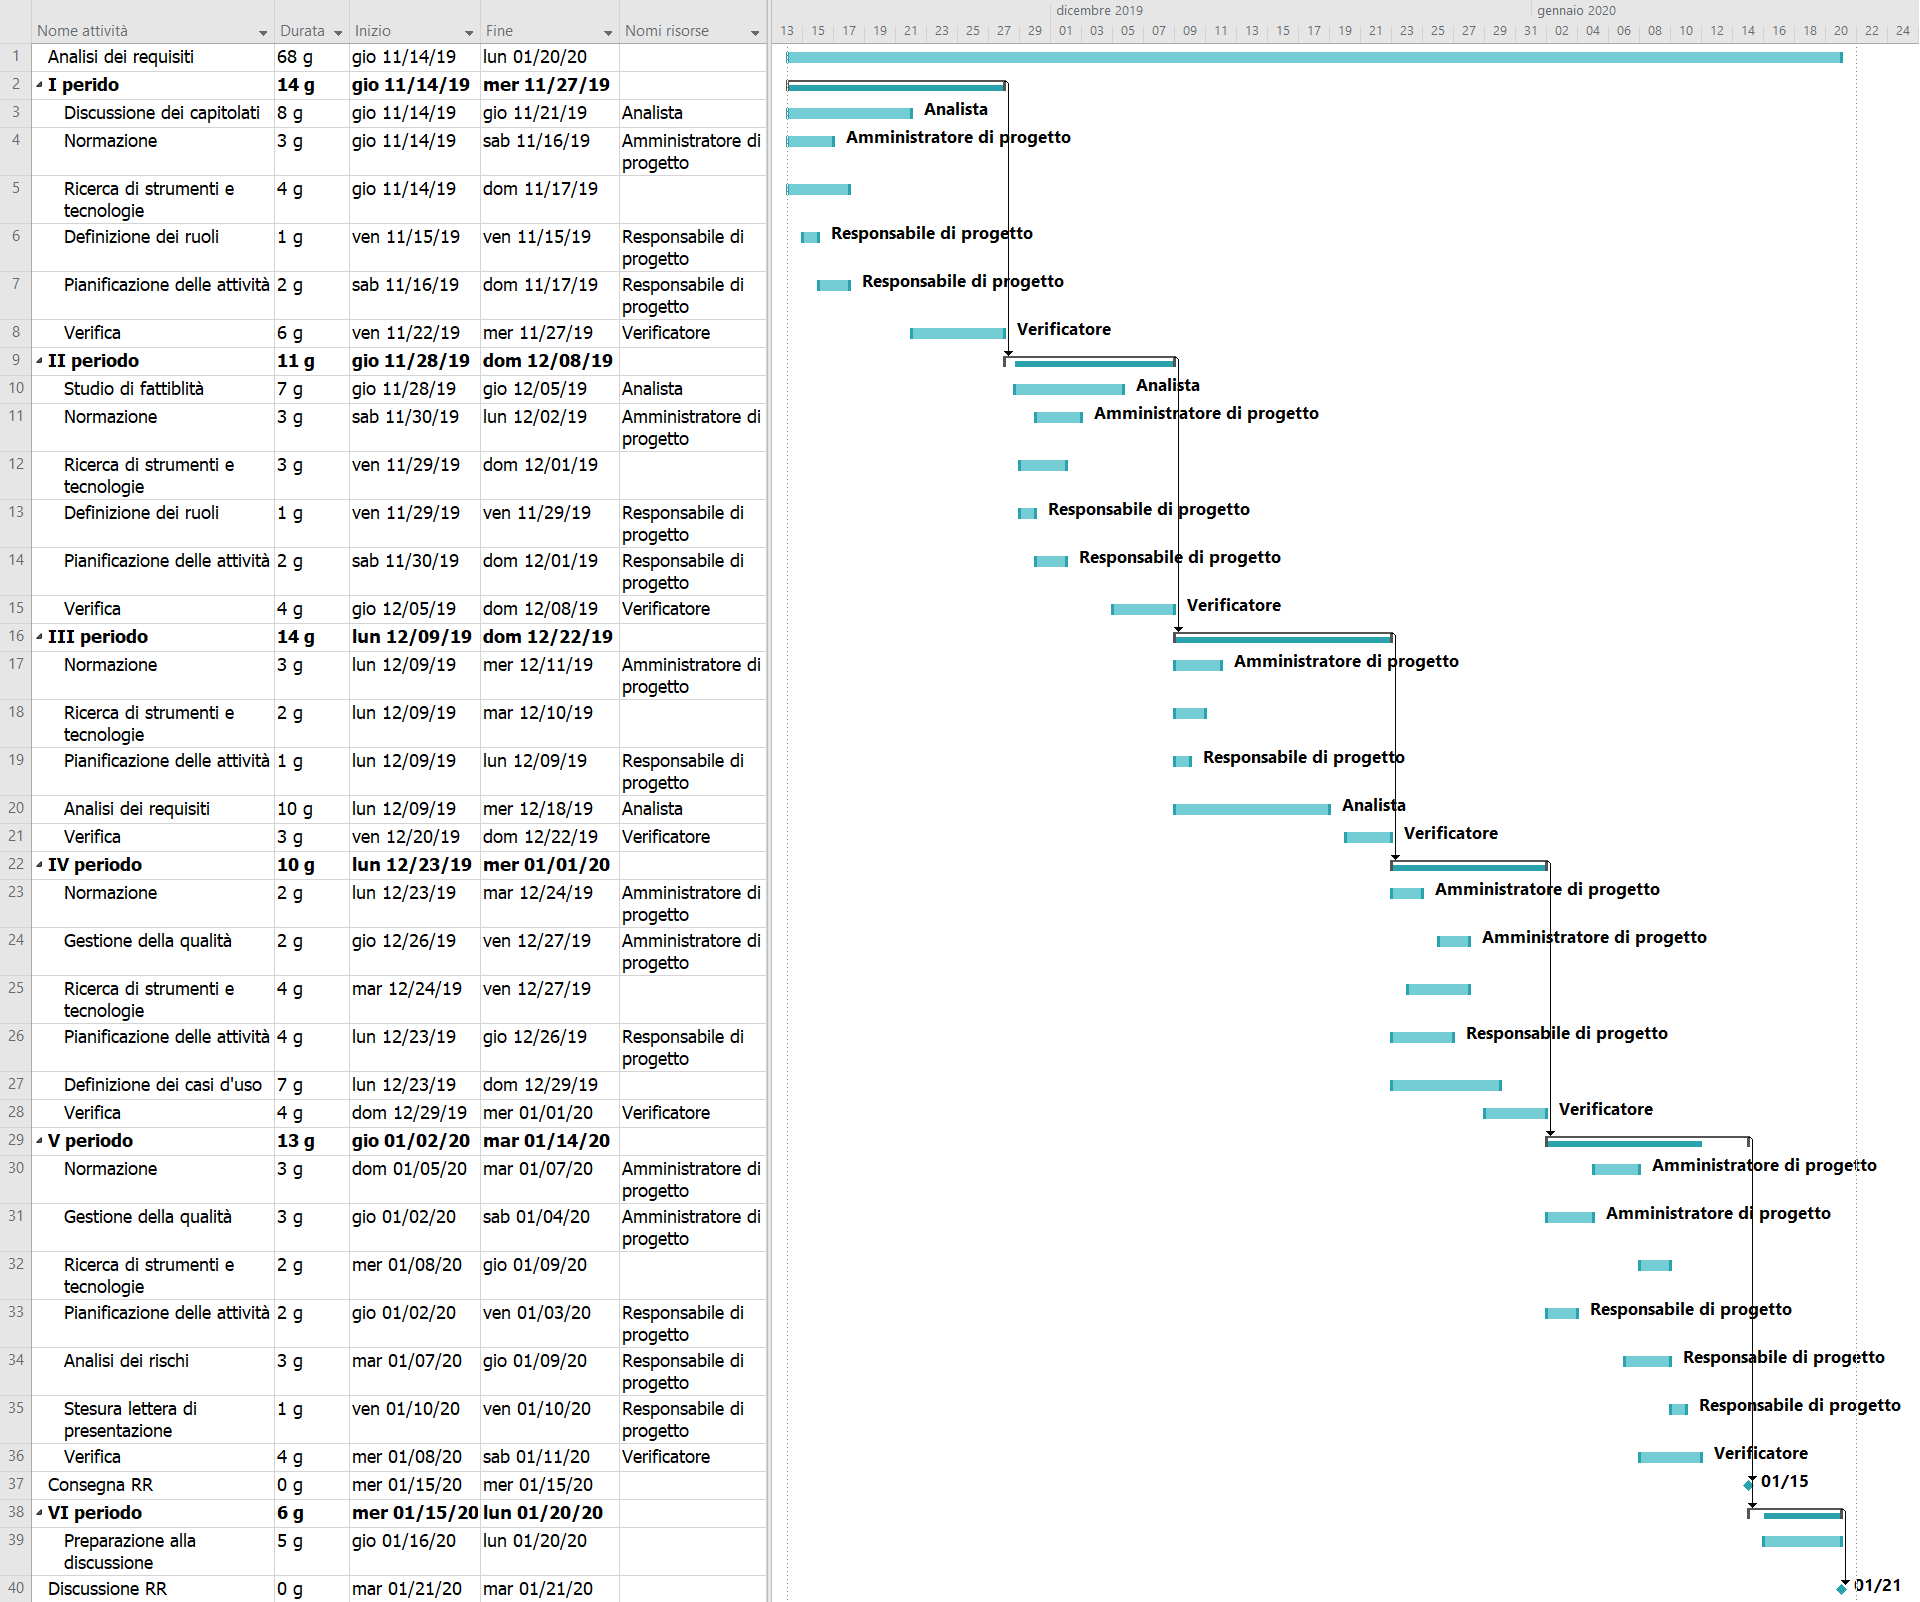
\includegraphics[width=\linewidth]{./gantt/Analisi dei requisiti.png}
	\caption{Diagramma di Gantt del periodo Analisi dei Requisiti}
\end{figure}
\pagebreak

\subsection{Progettazione architetturale}
La progettazione\glosp architetturale è il secondo macro periodo: inizia il 2020-01-22, giorno successivo alla prima revisione e finisce il 2020-02-20, giorno precedente alla seconda revisione. Durante questo macro periodo ci occuperemo della progettazione\glosp della codifica del codice del prodotto\glo.

\subsubsection{Ruoli attivi}
\begin{itemize}
	\item Responsabile di progetto\glo;
	\item amministratore di progetto\glo;
	\item analista;
	\item progettista;
	\item programmatore;
	\item verificatore.
\end{itemize}

\subsubsection{Periodi}
\paragraph*{I periodo: dal 2020-01-22 al 2020-02-09}
\begin{itemize}
	\item \textbf{Pianificazione delle attività}: gestione delle risorse disponibili, suddivisione e pianificazione di tutte le attività che devono essere svolte in questo periodo;
	\item \textbf{Normazione}: revisione e, se necessario, aggiornamento delle \textit{Norme di Progetto};
	\item \textbf{Gestione della qualità}: revisione delle metodologie per mantenere e garantire la qualità del prodotto\glo;
	\item \textbf{Revisione dei requisiti}: revisione ed, eventualmente, modifica dei requisiti analizzati durante la prima attività in seguito a modifiche di casi d'uso\glosp o di altre indicazioni;
	\item \textbf{Ricerca di strumenti e tecnologie}: ricerca delle tecnologie necessarie allo sviluppo del progetto\glo;
	\item \textbf{Verifica}: attività di controllo dei documenti modificati durante questo periodo.
\end{itemize}

\paragraph*{II periodo: dal 2020-02-10 al 2020-02-18}
\begin{itemize}
	\item \textbf{Pianificazione delle attività}: gestione delle risorse disponibili, suddivisione e pianificazione di tutte le attività che devono essere svolte in questo periodo;
	\item \textbf{Normazione}: revisione e aggiornamento delle \textit{Norme di Progetto};
	\item \textbf{Gestione della qualità}: revisione delle metodologie per mantenere e garantire la qualità del prodotto\glo;
	\item \textbf{Configurazione di strumenti e tecnologie}: configurazione delle tecnologie necessarie allo sviluppo del progetto\glo;
	\item \textbf{Revisione dei casi d'uso}\glo: revisione e modifica dei casi d'uso\glosp in seguito a indicazioni da parte del proponente;
	\item \textbf{Revisione dei requisiti}: revisione e modifica dei requisiti analizzati durante la prima attività in seguito a modifiche di casi d'uso\glosp o di altre indicazioni;
	\item \textbf{Progettazione}\glosp\textbf{proof of concept}\glo: pianificazione dello sviluppo di una proof of concept\glosp per dimostrare la fattibilità del prodotto\glo;
	\item \textbf{Verifica}: attività di controllo dei documenti modificati durante questo periodo.
\end{itemize}

\paragraph*{III periodo: dal 2020-02-19 al 2020-02-21}
\begin{itemize}
	\item \textbf{Normazione}: revisione e aggiornamento delle \textit{Norme di Progetto};
	\item \textbf{Pianificazione delle attività}: gestione delle risorse disponibili, suddivisione e pianificazione di tutte le attività che devono essere svolte in questo periodo;
	\item \textbf{Codifica proof of concept}\glo: sviluppo del codice per realizzare il proof of concept\glosp precedentemente pianificato, implementazione degli incrementi 1 e 9 del modello di sviluppo incrementale;
	\item \textbf{Stesura lettera di presentazione}: stesura della \textit{Lettera di Presentazione} in cui si propone una soluzione alla richiesta del proponente;
	\item \textbf{Verifica}: attività di controllo dei documenti e del codice sorgente realizzati durante questo periodo.
\end{itemize}

\paragraph*{IV periodo: dal 2020-02-22 al 2020-02-25}
\begin{itemize}
	\item \textbf{Pianificazione delle attività}: gestione delle risorse disponibili, suddivisione e pianificazione di tutte le attività che devono essere svolte in questo periodo;
	% Verificare se scrivere incremento 7 e 15 come parziali: nel PoC faremo solo esportazione del file e visualizzazione dei dati
	% Da incremento 7 eventualmente togliere "creazione"
	% Da incremento 15 eventualmente togliere "elaborazione"
	\item \textbf{Codifica proof of concept}\glo: sviluppo del codice per realizzare il proof of concept\glosp precedentemente pianificato, implementazione degli incrementi 2, 7, 12 e 15 del modello di sviluppo incrementale;
	\item \textbf{Verifica}: attività di controllo dei documenti e del codice sorgente realizzati durante questo periodo.
\end{itemize}

\paragraph*{V periodo: dal 2020-02-26 al 2020-03-08}
\begin{itemize}
	\item \textbf{Studio di strumenti e tecnologie}: revisione delle tecnologie e degli strumenti necessari per lo sviluppo del prodotto\glosp richiesto dal proponente in seguito alla presentazione dei PoC\glosp agli stakeholder\glo;
	\item \textbf{Normazione}: revisione e aggiornamento delle \textit{Norme di Progetto};
	\item \textbf{Pianificazione delle attività}: gestione delle risorse disponibili, suddivisione e pianificazione di tutte le attività che devono essere svolte in questo periodo;
	\item \textbf{Progettazione}\glosp\textbf{proof of concept}\glo: eventuale revisione della progettazione\glosp della proof of concept\glosp per dimostrare la fattibilità del prodotto\glo;
	\item \textbf{Codifica proof of concept}\glo: aggiornamento del codice del proof of concept\glosp in seguito alla presentazione agli stakeholder\glo;
	\item \textbf{Stesura lettera di presentazione}: stesura della \textit{Lettera di Presentazione} in cui si propone una soluzione alla richiesta del proponente;
	\item \textbf{Verifica}: attività di controllo dei documenti e del codice sorgente realizzati durante questo periodo.
\end{itemize}

\paragraph*{VI periodo: dal 2020-03-09 al 2020-03-15}
\begin{itemize}
	\item \textbf{Preparazione alla discussione}: realizzazione della presentazione e preparazione individuale e di gruppo alla discussione.
\end{itemize}

\begin{landscape}
	\begin{figure}
		\centering
		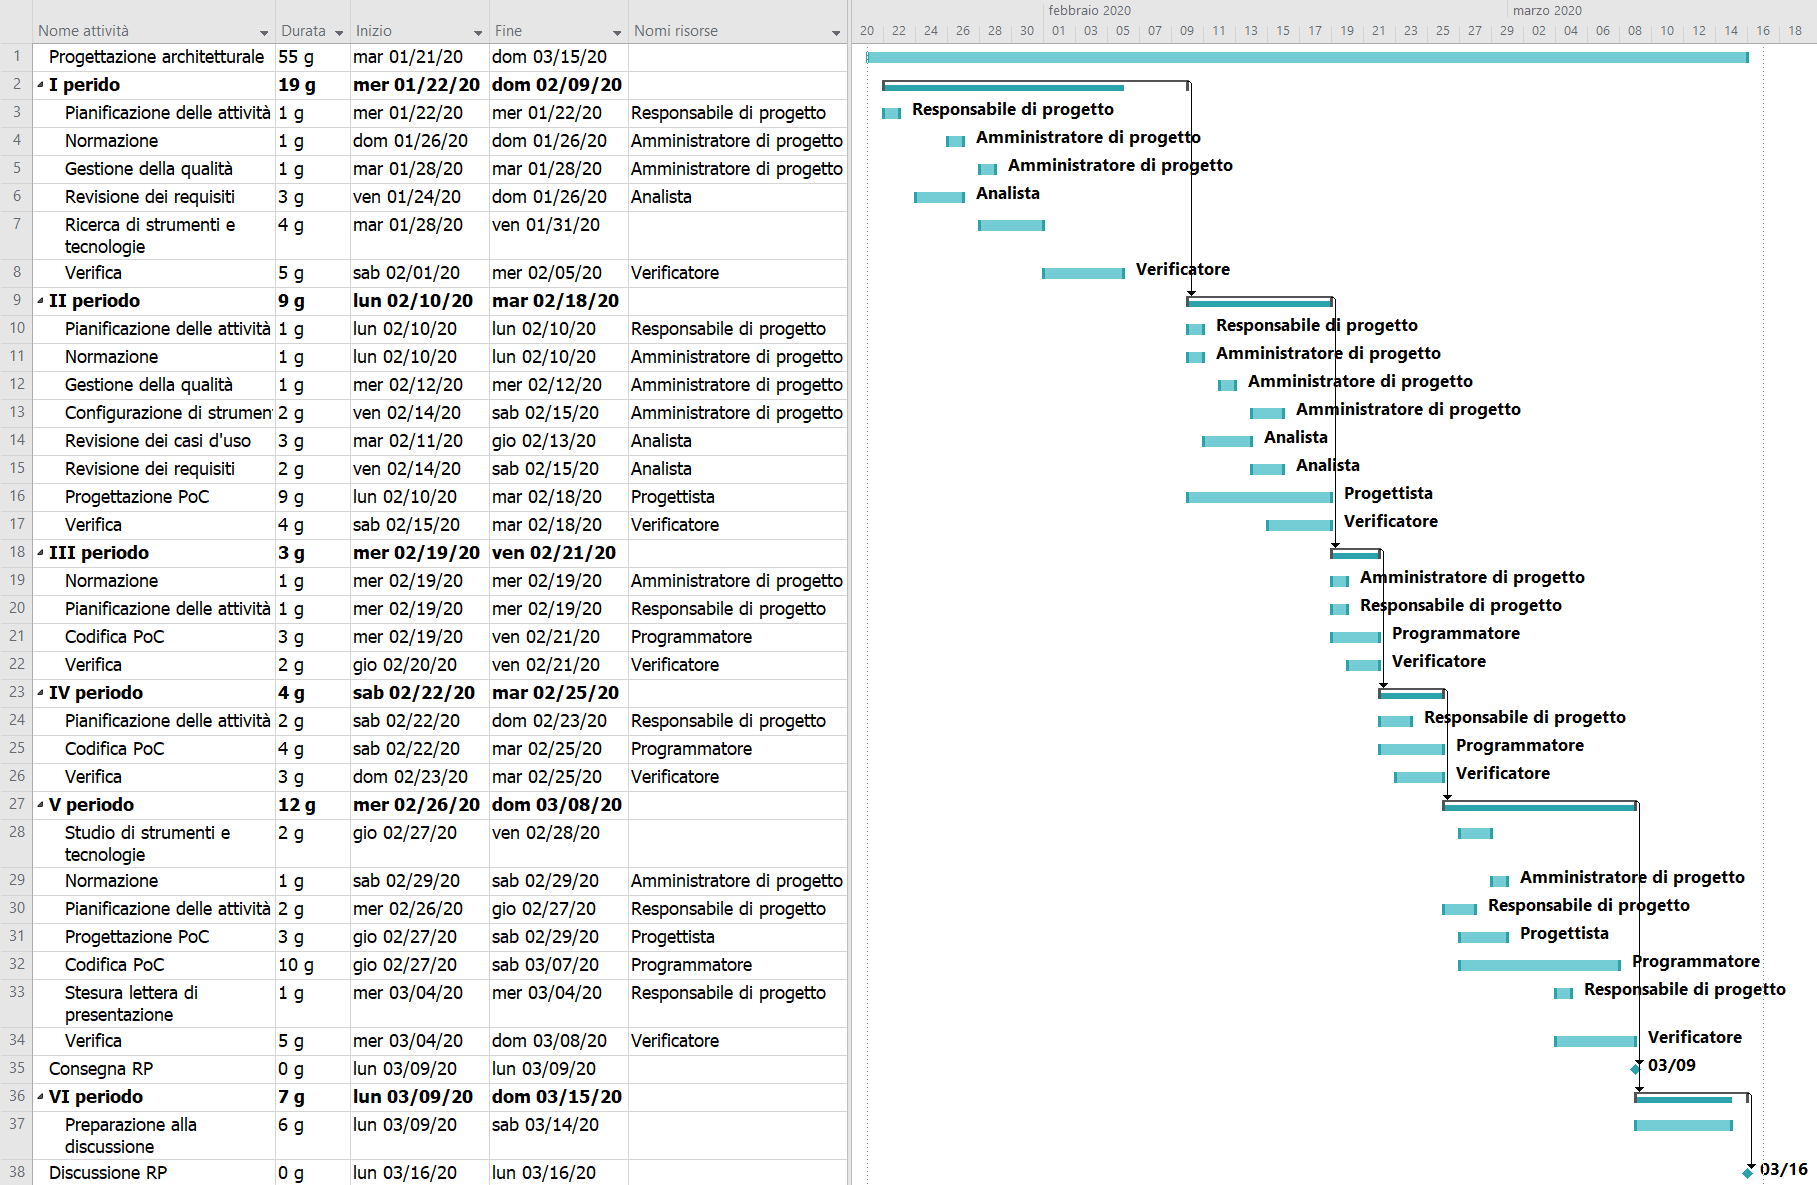
\includegraphics[scale=0.512]{./gantt/Progettazione architetturale.png}
		\caption{Diagramma di Gantt del periodo Progettazione Architetturale}
	\end{figure}
\end{landscape}
\pagebreak


\subsection{Progettazione di dettaglio e codifica}
La progettazione\glosp di dettaglio e codifica è il nostro terzo macro periodo: inizia il 2020-03-17, giorno successivo alla seconda revisione e finisce il 2020-04-19, giorno precedente alla terza revisione. Durante questo periodo ci occuperemo principalmente dell'attività di progettazione di dettaglio e di codifica del prodotto\glo. \\
In particolare ci poniamo i seguenti obiettivi:
\begin{itemize}
	\item revisione e aggiornamento dei documenti;
	\item revisione e aggiornamento della progettazione architetturale del prodotto\glosp software;
	\item definizione dell'architettura di dettaglio del prodotto\glosp software;
	\item stesura dell'allegato tecnico alla Product Baseline\glo;
	\item stesura del \textit{Manuale dello sviluppatore};
	\item implementazione degli incrementi necessari a garantire la presenza delle funzionalità fondamentali del prodotto. In particolare:
		\begin{itemize}
		\item incremento 3;
		\item incremento 4;
		\item incremento 6;
		\item incremento 13;
		\item incremento 14;
		\item incremento 16.
		\end{itemize}
	\item verifica di quanto implementato;
	\item stesura del \textit{Manuale Utente} sulla base degli incrementi sviluppati;
	\item conseguimento del colloquio per la Product Baseline\glosp con il committente;
	\item realizzazione della presentazione e preparazione alla discussione.
\end{itemize}
Al termine di questo periodo ci aspettiamo quindi di avere un prodotto\glosp di qualità che fornisca le funzionalità fondamentali e con un livello di copertura dei test accettabile. 
\subsubsection*{Ruoli attivi}
\begin{itemize}
	\item Responsabile di progetto\glo;
	\item amministratore di progetto\glo;
	\item analista;
	\item progettista;
	\item programmatore;
	\item verificatore.
\end{itemize}
Di seguito analizziamo la pianificazione di dettaglio per quanto concerne lo sviluppo di ciascun incremento.

\subsubsection{Incremento 3}
\textbf{I periodo: dal 2020-03-17 al 2020-03-24} \\ 
L'incremento 3 prevede lo sviluppo e l'implementazione dell'algoritmo di addestramento SVM\glosp nell'applicazione di addestramento e nel plug-in. 
\\Prevede il soddisfacimento completo o parziale dei seguenti requisiti:
\begin{itemize}
	\item R1F4.2;
	\item R1F4.10;
	\item R1F11;
	\item R2F4.6.
\end{itemize}
Viene svolto in un unico periodo.
\paragraph{Ruoli attivi}
\begin{itemize}
	\item Responsabile di progetto\glo;
	\item amministratore di progetto\glo;
	\item analista
	\item progettista;
	\item programmatore;
	\item verificatore.
\end{itemize}
\paragraph{Attività} 
\begin{itemize}
	\item \textbf{Revisione dei documenti}: revisione e, se necessario, aggiornamento dei documenti secondo le indicazioni del committente;
	\item \textbf{Normazione}: revisione e, se necessario, aggiornamento delle \textit{Norme di Progetto};
	\item \textbf{Ricerca di strumenti e tecnologie}: ricerca e studio degli strumenti e tecnologie utilizzate per la codifica;
	\item \textbf{Pianificazione delle attività}: gestione delle risorse disponibili, suddivisione e pianificazione di tutte le attività che devono essere svolte in questo periodo;
	\item \textbf{Progettazione}\glo: definizione in modo più dettagliato ed eventuali correzioni dell'architettura del nostro prodotto\glosp software con rispettiva individuazione dei design pattern architetturali da applicare e progettazione\glosp dell'incremento 3; 
	\item \textbf{Revisione dei requisiti}: revisione ed, eventualmente, modifica dei requisiti analizzati secondo le indicazioni; 
	\item \textbf{Codifica}: scrittura del codice del prodotto\glosp seguendo le indicazioni definite nel documento \textit{Norme di Progetto} e nella progettazione\glosp indicata sopra. Codifica per l'implementazione dell'incremento 3; 
	\item \textbf{Verifica}: attività di controllo dei documenti e del codice realizzati durante questo periodo.
\end{itemize}
\subsubsection{Incremento 4}
\textbf{II periodo: dal 2020-03-25 al 2020-03-30} \\
L'incremento 4 prevede lo sviluppo e l'implementazione dell'algoritmo di addestramento RL\glosp nell'applicazione di addestramento e nel plug-in.
\\Prevede il soddisfacimento completo o parziale dei seguenti requisiti:
\begin{itemize}
	\item R1F4.2;
	\item R1F4.11. 
\end{itemize}
Viene svolto in un unico periodo.
\paragraph{Ruoli attivi}
\begin{itemize}
	\item Responsabile di progetto\glo;
	\item amministratore di progetto\glo;
	\item analista
	\item progettista;
	\item programmatore;
	\item verificatore.
\end{itemize}
\paragraph{Attività} 
\begin{itemize}
	\item \textbf{Normazione}: revisione e, se necessario, aggiornamento delle \textit{Norme di Progetto};
	\item \textbf{Ricerca di strumenti e tecnologie}: ricerca e studio degli strumenti e tecnologie utilizzate per la codifica;
	\item \textbf{Pianificazione delle attività}: gestione delle risorse disponibili, suddivisione e pianificazione di tutte le attività che devono essere svolte in questo periodo;
	\item \textbf{Progettazione}\glo: revisione e aggiornamento della progettazione\glosp dell'architettura del prodotto\glosp con rispettiva individuazione dei design pattern architetturali da applicare e progettazione\glosp dell'incremento 4; 
	\item \textbf{Revisione dei requisiti}: revisione ed, eventualmente, modifica dei requisiti analizzati secondo le indicazioni; 
	\item \textbf{Codifica}: scrittura del codice del prodotto\glosp seguendo le indicazioni definite nel documento \textit{Norme di Progetto} e nella progettazione\glosp indicata sopra. Codifica per l'implementazione dell'incremento 4;
	\item \textbf{Scrittura manuale sviluppatore}: inizio della scrittura del \textit{Manuale dello sviluppatore} per fornire le indicazioni utili ad uno sviluppatore che vuole contribuire al progetto\glo; 
	\item \textbf{Verifica}: attività di controllo dei documenti e del codice realizzati durante questo periodo.
\end{itemize}
\subsubsection{Incremento 6}
\textbf{III periodo: dal 2020-03-31 al 2020-04-02} \\
L'incremento 6 prevede lo sviluppo e l'implementazione della funzionalità che permette all'utente di selezionare un modello di predizione e avviare l'addestramento dello stesso.
\\Prevede il soddisfacimento completo o parziale dei seguenti requisiti:
\begin{itemize}
	\item R1F4.4;
	\item R1F4.11;
	\item R1F4.12.
\end{itemize}
Viene svolto in un unico periodo.
\paragraph{Ruoli attivi}
\begin{itemize}
	\item Responsabile di progetto\glo;
	\item amministratore di progetto\glo;
	\item progettista;
	\item programmatore;
	\item verificatore.
\end{itemize}
\paragraph{Attività} 
\begin{itemize}
	\item \textbf{Normazione}: revisione e, se necessario, aggiornamento delle \textit{Norme di Progetto};
	\item \textbf{Ricerca di strumenti e tecnologie}: ricerca e studio degli strumenti e tecnologie utilizzate per la codifica;
	\item \textbf{Pianificazione delle attività}: gestione delle risorse disponibili, suddivisione e pianificazione di tutte le attività che devono essere svolte in questo periodo;
	\item \textbf{Progettazione}\glo: progettazione\glosp dell'incremento 6;  
	\item \textbf{Codifica}: scrittura del codice del prodotto\glosp seguendo le indicazioni definite nel documento \textit{Norme di Progetto} e nella progettazione\glosp indicata sopra. Codifica per l'implementazione dell'incremento 6;
	\item \textbf{Scrittura manuale sviluppatore}: aggiornamento del \textit{Manuale dello sviluppatore};
	\item \textbf{Verifica}: attività di controllo dei documenti e del codice realizzati durante questo periodo.
\end{itemize}
\subsubsection{Incremento 13}
\textbf{IV periodo: dal 2020-04-03 al 2020-04-05} \\
L'incremento 13 prevede lo sviluppo e l'implementazione della lettura del file di configurazione, che sarà in formato JSON, e la conseguente configurazione degli algoritmi.
\\Prevede il soddisfacimento completo o parziale dei seguenti requisiti:
\begin{itemize}
	\item R1F8;
	\item R1F11.
\end{itemize}
Viene svolto in un unico periodo.
\paragraph{Ruoli attivi}
\begin{itemize}
	\item Responsabile di progetto\glo;
	\item amministratore di progetto\glo;
	\item progettista;
	\item programmatore;
	\item verificatore.
\end{itemize}
\paragraph{Attività} 
\begin{itemize}
	\item \textbf{Normazione}: revisione e, se necessario, aggiornamento delle \textit{Norme di Progetto};
	\item \textbf{Pianificazione delle attività}: gestione delle risorse disponibili, suddivisione e pianificazione di tutte le attività che devono essere svolte in questo periodo;
	\item \textbf{Progettazione}\glo: progettazione\glosp dell'incremento 13;  
	\item \textbf{Codifica}: scrittura del codice del prodotto\glosp seguendo le indicazioni definite nel documento \textit{Norme di Progetto} e nella progettazione\glosp indicata sopra. Codifica per l'implementazione dell'incremento 13;
	\item \textbf{Scrittura manuale sviluppatore}: aggiornamento del \textit{Manuale dello sviluppatore};
	\item \textbf{Scrittura manuale utente}: inizio della scrittura del \textit{Manuale utente} per descrivere come deve l'utente finale deve utilizzare il software;
	\item \textbf{Verifica}: attività di controllo dei documenti e del codice realizzati durante questo periodo.
\end{itemize}
\subsubsection{Incremento 14}
\textbf{V periodo: dal 2020-04-06 al 2020-04-10} \\
L'incremento 14 prevede lo sviluppo e l'implementazione dell'associazione dei nodi al flusso dati e dell'elaborazione e visualizzazione dei dati.
\\Prevede il soddisfacimento completo o parziale dei seguenti requisiti:
\begin{itemize}
	\item R1F9;
	\item R1F9.1;
	\item R1F9.2;
	\item R1F9.4;
	\item R1F9.5;
	\item R1F11.
\end{itemize}
Viene svolto in un unico periodo.
\paragraph{Ruoli attivi}
\begin{itemize}
	\item Responsabile di progetto\glo;
	\item amministratore di progetto\glo;
	\item progettista;
	\item programmatore;
	\item verificatore.
\end{itemize}
\paragraph{Attività} 
\begin{itemize}
	\item \textbf{Normazione}: revisione e, se necessario, aggiornamento delle \textit{Norme di Progetto};
	\item \textbf{Pianificazione delle attività}: gestione delle risorse disponibili, suddivisione e pianificazione di tutte le attività che devono essere svolte in questo periodo;
	\item \textbf{Progettazione}\glo: progettazione\glosp dell'incremento 14;  
	\item \textbf{Codifica}: scrittura del codice del prodotto\glosp seguendo le indicazioni definite nel documento \textit{Norme di Progetto} e nella progettazione\glosp indicata sopra. Codifica per l'implementazione dell'incremento 14;
	\item \textbf{Scrittura manuale sviluppatore}: aggiornamento del \textit{Manuale dello sviluppatore};
	\item \textbf{Scrittura manuale utente}: aggiornamento del \textit{Manuale utente};
	\item \textbf{Verifica}: attività di controllo dei documenti e del codice realizzati durante questo periodo.
\end{itemize}
\subsubsection{Incremento 16}
\textbf{VI periodo: dal 2020-04-11 al 2020-04-13} \\
L'incremento 16 prevede lo sviluppo e l'implementazione della funzionalità che permette all'utente di arrestare l'algoritmo di addestramento prima del suo termine naturale.
\\Prevede il soddisfacimento completo o parziale dei seguenti requisiti:
\begin{itemize}
	\item R1F12;
	\item R1F20.
\end{itemize}
Viene svolto in un unico periodo.
\paragraph{Ruoli attivi}
\begin{itemize}
	\item Responsabile di progetto\glo;
	\item amministratore di progetto\glo;
	\item progettista;
	\item programmatore;
	\item verificatore.
\end{itemize}
\paragraph{Attività} 
\begin{itemize}
	\item \textbf{Normazione}: revisione e, se necessario, aggiornamento delle \textit{Norme di Progetto};
	\item \textbf{Pianificazione delle attività}: gestione delle risorse disponibili, suddivisione e pianificazione di tutte le attività che devono essere svolte in questo periodo;
	\item \textbf{Progettazione}\glo: progettazione\glosp dell'incremento 16;  
	\item \textbf{Codifica}: scrittura del codice del prodotto\glosp seguendo le indicazioni definite nel documento \textit{Norme di Progetto} e nella progettazione\glosp indicata sopra. Codifica per l'implementazione dell'incremento 16;
	\item \textbf{Scrittura manuale sviluppatore}: chiusura del \textit{Manuale dello sviluppatore};
	\item \textbf{Scrittura manuale utente}: chiusura del \textit{Manuale utente};
	\item \textbf{Stesura lettera di presentazione}: stesura della \textit{Lettera di Presentazione} in cui si propone una soluzione alla richiesta del proponente;
	\item \textbf{Verifica}: attività di controllo dei documenti e del codice realizzati durante questo periodo.
\end{itemize}
\subsubsection{VII periodo: dal 2020-04-14 al 2020-04-19}
Durante questo periodo è prevista la preparazione alla discussione della revisione di qualifica.
\paragraph{Ruoli attivi} \mbox{}\\ [1mm]
Non è previsto alcun ruolo attivo.
\paragraph{Attività}

\begin{itemize}
	\item \textbf{Preparazione alla discussione}: realizzazione della presentazione e preparazione individuale e di gruppo alla discussione.
\end{itemize}

\begin{figure}
	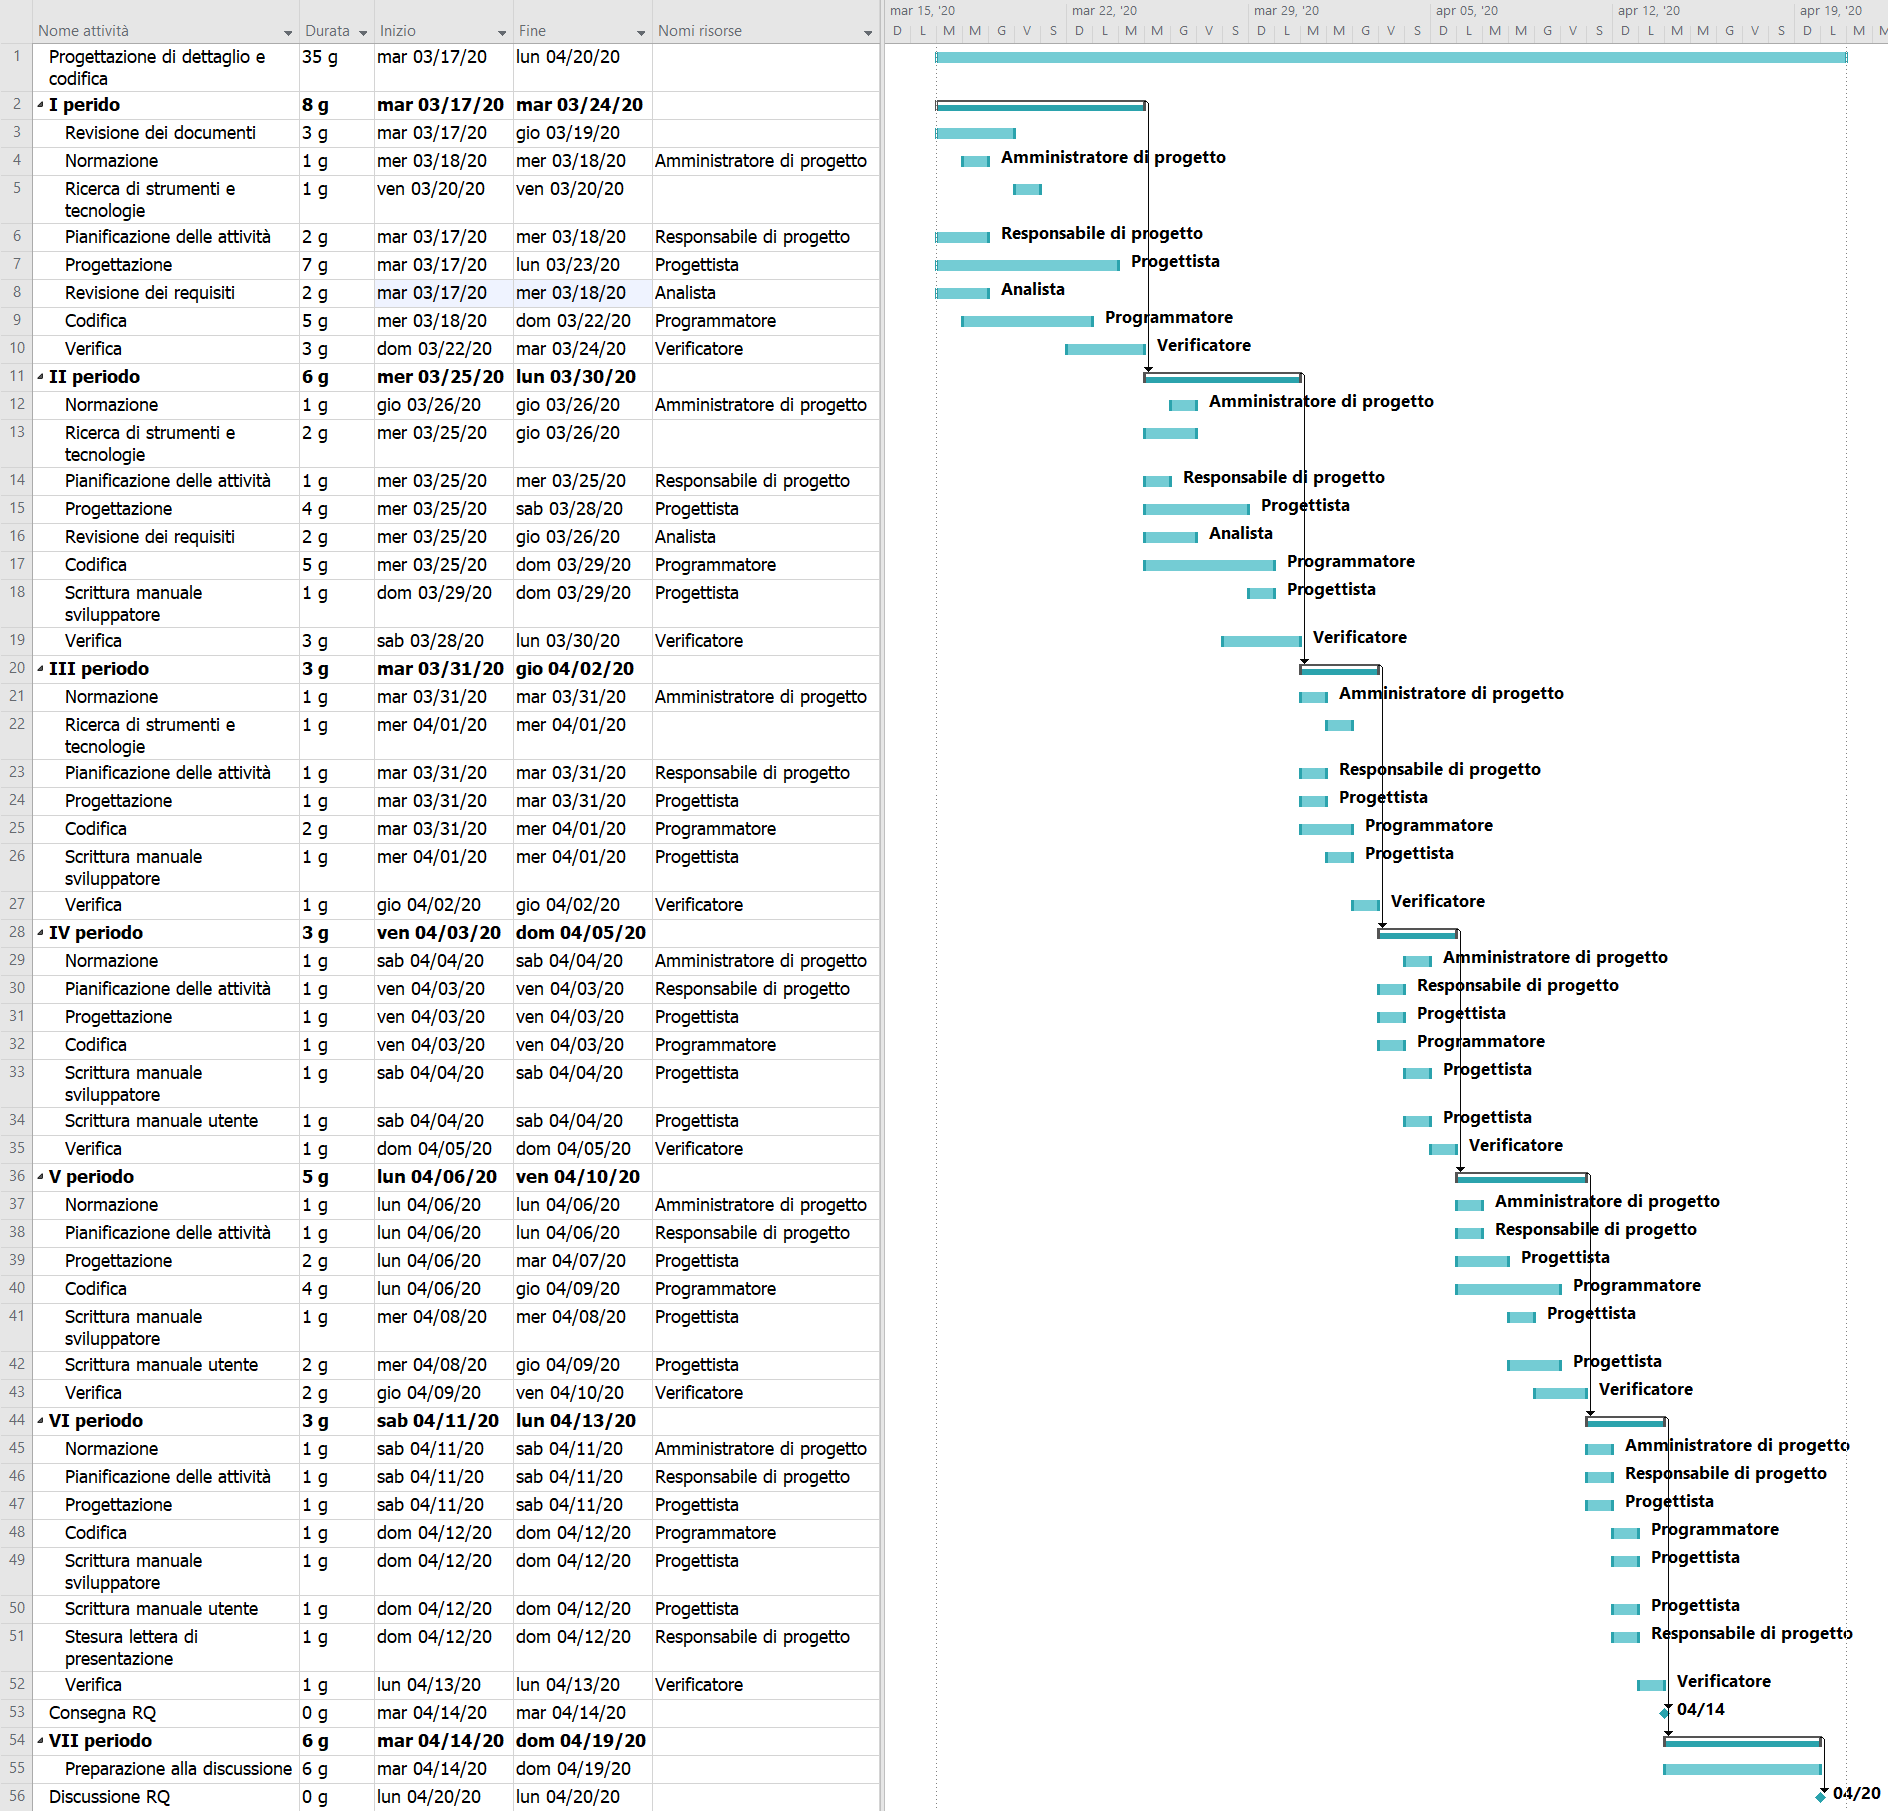
\includegraphics[width=\linewidth]{./gantt/Progettazione di dettaglio e codifica.png}
	\caption{Diagramma di Gantt del periodo Progettazione di dettaglio e codifica}
\end{figure}
\pagebreak

\subsection{Validazione e collaudo}
Validazione\glosp e collaudo è il nostro quarto macro periodo: inizia il 2020-04-21, giorno successivo alla terza revisione e si conclude il 2020-05-17, giorno precedente all'ultima revisione. Durante questo macro periodo ci occuperemo dello sviluppo di due incrementi che completano il nostro prodotto e del collaudo e della validazione\glosp dello stesso. per verificare che tutti i requisiti definiti come obbligatori nell'\textit{Analisi dei Requisiti} siano stati soddisfatti. \\
In particolare per questo periodo ci poniamo i seguenti obiettivi:
\begin{itemize}
	\item revisione e aggiornamento dei documenti;	
	\item implementazione degli incrementi rimanenti per completare le funzionalità del prodotto\glosp previste. In particolare:
		\begin{itemize}
			\item incremento 8;
			\item incremento 17.
		\end{itemize}
	\item verifica di quanto implementato;
	\item aggiornamento del \textit{Manuale dello sviluppatore};
	\item aggiornamento del \textit{Manuale Utente};
	\item realizzazione della presentazione e preparazione alla discussione.	
\end{itemize}
Al termine di questo periodo ci aspettiamo quindi di avere un prodotto\glosp di qualità completo, con un livello di copertura dei test accettabile e approvato dal proponente. 

\subsubsection*{Ruoli attivi}
\begin{itemize}
	\item Responsabile di progetto\glo;
	\item amministratore di progetto\glo;
	\item progettista;
	\item programmatore;
	\item verificatore.
\end{itemize}

Di seguito analizziamo la pianificazione di dettaglio per quanto concerne lo sviluppo di ciascun incremento e le attività di correzione e chiusura finale dei documenti.

\subsubsection{Incremento 8}
\textbf{I periodo: dal 2020-04-21 al 2020-04-28} \\
L'incremento 8 prevede lo sviluppo e l'implementazione della funzionalità di visualizzazione degli indici di qualità dell'addestramento degli algoritmi.
\\Prevede il soddisfacimento completo o parziale dei seguenti requisiti:
\begin{itemize}
	\item R1F5;
	\item R1F5.1;
	\item R1F5.2;
	\item R1F5.3.
\end{itemize}
Viene svolto in un unico periodo.
\paragraph{Ruoli attivi}
\begin{itemize}
	\item Responsabile di progetto\glo;
	\item amministratore di progetto\glo;
	\item progettista;
	\item programmatore;
	\item verificatore.
\end{itemize}
\paragraph{Attività}
\begin{itemize}
	\item \textbf{Normazione}: revisione e, se necessario, aggiornamento delle \textit{Norme di Progetto};
	\item \textbf{Pianificazione delle attività}: gestione delle risorse disponibili, suddivisione e pianificazione di tutte le attività che devono essere svolte in questo periodo;
	\item \textbf{Progettazione}: progettazione di dettaglio dell'incremento 8;
	\item \textbf{Codifica}: implementazione dell'incremento 8 seguendo le indicazioni delle \textit{Norme di Progetto} e della progettazione\glosp indicata sopra;
	\item \textbf{Test e collaudo}: scrittura dei test mancanti per il collaudo finale del prodotto\glo;
	\item \textbf{Verifica}: attività di controllo del codice e dei documenti realizzati durante questo periodo.
\end{itemize}

\subsubsection{Incremento 17}
\textbf{II periodo: dal 2020-04-29 al 2020-05-02} \\
L'incremento 17 prevede lo sviluppo e l'implementazione della funzionalità di visualizzazione degli errori in caso di inserimento di file non validi e errata mappatura dei predittori con il flusso di dati ricevuto dalla datasource.
\\Prevede il soddisfacimento completo o parziale dei seguenti requisiti:
\begin{itemize}
	\item R2F6;
	\item R2F10;
	\item R2F18.
\end{itemize}
Viene svolto in un unico periodo.
\paragraph{Ruoli attivi}
\begin{itemize}
	\item Responsabile di progetto\glo;
	\item amministratore di progetto\glo;
	\item progettista;
	\item programmatore;
	\item verificatore.
\end{itemize}
\paragraph{Attività}
\begin{itemize}
	\item \textbf{Normazione}: revisione e, se necessario, aggiornamento delle \textit{Norme di Progetto};
	\item \textbf{Pianificazione delle attività}: gestione delle risorse disponibili, suddivisione e pianificazione di tutte le attività che devono essere svolte in questo periodo;
	\item \textbf{Progettazione}: progettazione di dettaglio dell'incremento 17;
	\item \textbf{Manuale utente}: integrazione delle nuove funzionalità del prodotto\glo;
	\item \textbf{Manuale sviluppatore}:  revisione e, se necessario, aggiornamento del \textit{Manuale dello Sviluppatore};
	\item \textbf{Codifica}: implementazione dell'incremento 17 seguendo le indicazioni delle \textit{Norme di Progetto} e della progettazione\glosp indicata sopra;
	\item \textbf{Test e collaudo}: scrittura dei test mancanti per il collaudo finale del prodotto\glo;
	\item \textbf{Verifica}: attività di controllo del codice e dei documenti realizzati durante questo periodo.
\end{itemize}

\subsubsection{III periodo: dal 2020-05-03 al 2020-05-10}
Durante questo periodo è prevista la correzione e la chiusura di tutti i documenti.
\paragraph{Ruoli attivi}
\begin{itemize}
	\item Responsabile di progetto\glo;
	\item amministratore di progetto\glo;
	\item progettista;
	\item programmatore;
	\item verificatore.
\end{itemize}
\paragraph{Attività}
\begin{itemize}
	\item \textbf{Norme di progetto}: revisione e, se necessario, aggiornamento delle \textit{Norme di Progetto};
	\item \textbf{Pianificazione delle attività}: gestione delle risorse disponibili, suddivisione e pianificazione di tutte le attività che devono essere svolte in questo periodo;
	\item \textbf{Revisione dei documenti}: revisione e, se necessario, aggiornamento dei documenti secondo le indicazioni del committente;
	\item \textbf{Codifica}: codifica dei rimanenti test per il collaudo del prodotto\glosp ed eventuali bug fix;
	\item \textbf{Test e collaudo}: esecuzione finale dei test per il collaudo del prodotto\glo;
	\item \textbf{Verifica}: attività di controllo dei documenti e del codice realizzati durante questo periodo;
	\item \textbf{Stesura lettera di presentazione}: stesura della \textit{Lettera di Presentazione} che in cui si propone una soluzione alla richiesta del proponente.
\end{itemize}

\subsubsection{IV periodo: dal 2020-05-11 al 2020-05-17}
Durante questo periodo è prevista la preparazione alla discussione finale.
\paragraph{Ruoli attivi} \mbox{}\\ [1mm]
Non è previsto alcun ruolo attivo.
\paragraph{Attività}

\begin{itemize}
	\item \textbf{Preparazione alla discussione}: realizzazione della presentazione e preparazione individuale e di gruppo alla discussione.
\end{itemize}

\begin{landscape}
	\begin{figure}
		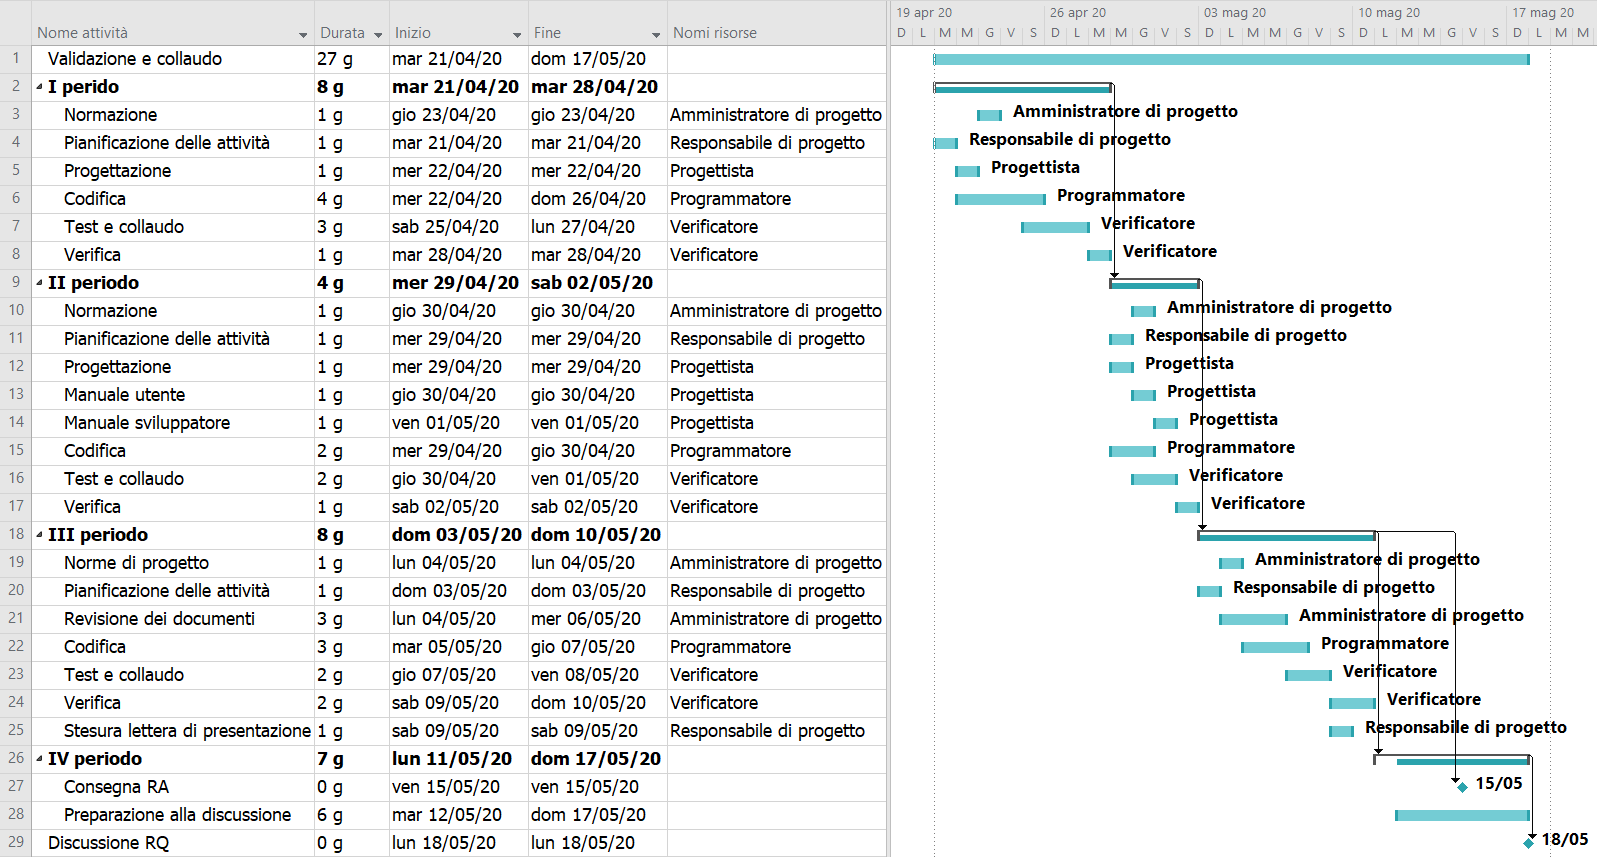
\includegraphics[width=\linewidth]{./gantt/Validazione e collaudo.png}
		\caption{Diagramma di Gantt del periodo Validazione e collaudo}
	\end{figure}
\end{landscape}
\pagebreak

	\pagebreak
	\section{Preventivo} %Meccanismi di controllo e rendicontazione
Viene in seguito presentato il preventivo del costo del lavoro da svolgere con i dettagli sul costo di ogni singolo periodo.
Per identificare i diversi ruoli verranno utilizzate le sigle:
\begin{itemize}
	\item \textbf{Re}: responsabile di progetto\glo;
	\item \textbf{Am}: amministratore di progetto\glo;
	\item \textbf{An}: analista;
	\item \textbf{Pt}: progettista;
	\item \textbf{Pr}: programmatore;
	\item \textbf{Ve}: verificatore.
\end{itemize}
	\subsection{Periodo di analisi}
	Le ore indicate per questo periodo vengono riportate solo perché utili ai fini del documento, non saranno rendicontate nel budget finale richiesto in quanto il periodo di analisi è da considerare come investimento per il gruppo.
	\pagebreak
		\subsubsection{Prospetto orario}
		Nel periodo di analisi è prevista la seguente divisione oraria:
		\begin{longtable} {				
				>{}p{40mm}  
				>{}p{8mm}
				>{}p{8mm}
				>{}p{8mm}
				>{}p{8mm}
				>{}p{8mm}
				>{}p{8mm}
				>{}p{12mm}				
			}			
			\rowcolor{gray!50}
			\textbf{Nominativo} & \textbf{Re} & \textbf{Am} & \textbf{An} & \textbf{Pt} & \textbf{Pr} & \textbf{Ve} & \textbf{Totale}	\TBstrut \\ [2mm]
			Corrizzato Vittorio & 6 & 6 & 8 & - & - & 5 & 25 \TBstrut \\ [2mm]
			Dalla Libera Marco & 7 & - & 13 & - & - & 5 & 25 \TBstrut \\ [2mm]
			Rampazzo Marco & - & 8 & 12 & - & - & 5 & 25 \TBstrut \\ [2mm]
			Santagiuliana Vittorio & - & 5 & 12 & - & - & 8 & 25 \TBstrut \\ [2mm]
			Schiavon Rebecca & - & - & 15 & - & - & 10 & 25 \TBstrut \\ [2mm]
			Spreafico Alessandro & - & - & 12 & 5 & - & 8 & 25 \TBstrut \\ [2mm]
			Toffoletto Massimo & 8 & 7 & 5 & - & - & 5 & 25 \TBstrut \\ [2mm]
			\rowcolor{white}
			\caption{Prospetto orario del periodo di analisi}
		\end{longtable}
		Rappresentata nel seguente grafico:
		\begin{figure} [H]
			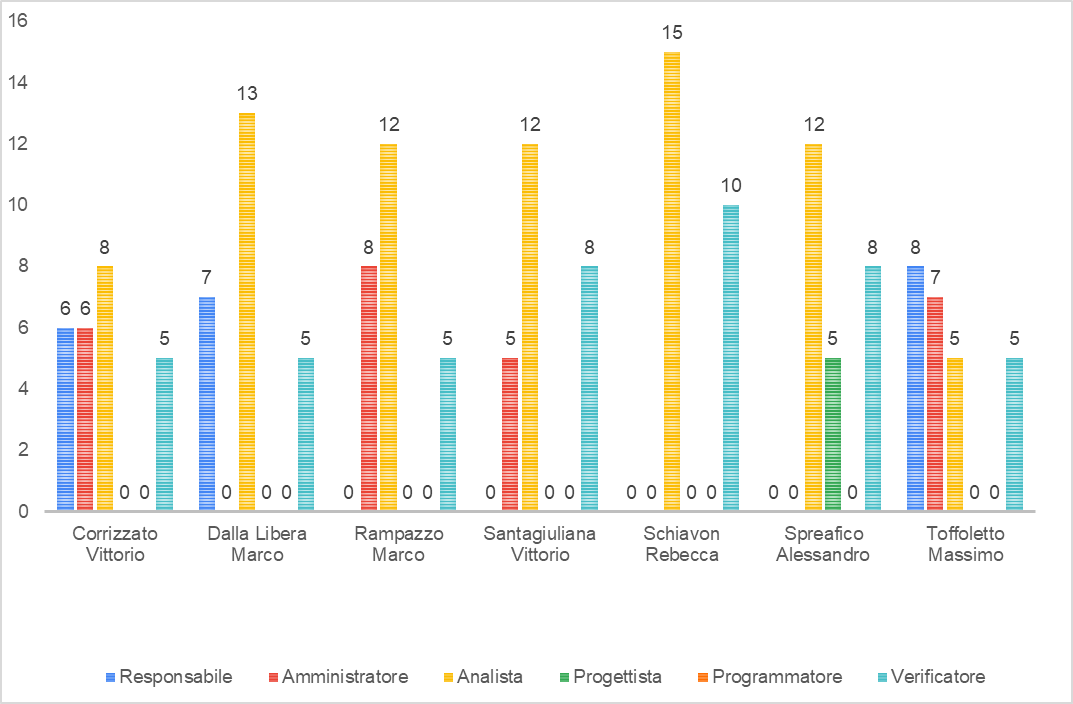
\includegraphics[width=\linewidth]{./img/Grafici/1.png}
			\caption{Grafico del prospetto orario del periodo di analisi}
		\end{figure}
	
		\subsubsection{Prospetto economico}
		Nel periodo di analisi sono previsti i seguenti costi:
		\begin{longtable} {
			>{}p{32mm}
			>{}p{20mm}
			>{}p{20mm}
		}
		\rowcolor{gray!50}
		
		\textbf{Ruolo} & \textbf{Ore} & \textbf{Costo} \TBstrut \\
		Responsabile & 21 & 630,00\euro{} \TBstrut \\
		Amministratore & 26 & 520,00\euro{} \TBstrut \\
		Analista & 77 & 1925,00\euro{} \TBstrut \\
		Progettista & 5 & 110,00\euro{} \TBstrut \\
		Programmatore & 0 & 0,00\euro{} \TBstrut \\
		Verificatore & 46 & 690,00\euro{} \TBstrut \\
		\textbf{Totale} & \textbf{175}& \textbf{3875,00\euro{}} \TBstrut \\
		\rowcolor{white}
		\caption{Prospetto economico del periodo di analisi}		
		\end{longtable}
		Rappresentati nel seguente grafico:
		\begin{figure} [H]
			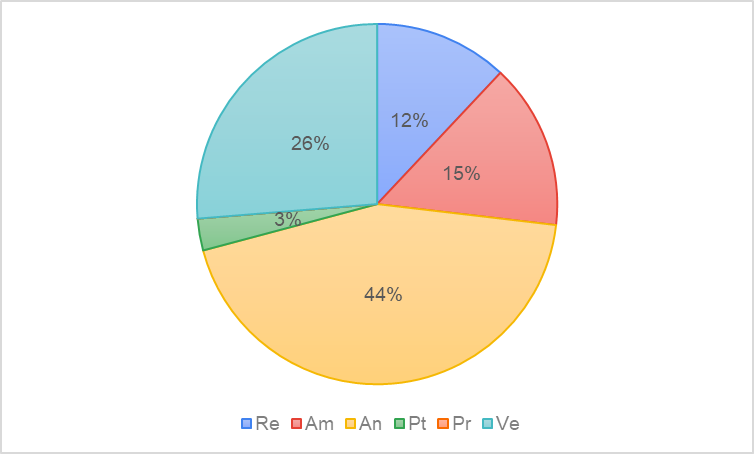
\includegraphics[width=\linewidth]{./img/Grafici/2.png}
			\caption{Grafico del prospetto economico del periodo di analisi}
		\end{figure}
\subsection{Periodo di progettazione architetturale}
	\subsubsection{Prospetto orario}
	Nel periodo di progettazione\glosp architetturale è prevista la seguente divisione oraria:
	\begin{longtable} {				
		>{}p{40mm}  
		>{}p{8mm}
		>{}p{8mm}
		>{}p{8mm}
		>{}p{8mm}
		>{}p{8mm}
		>{}p{8mm}
		>{}p{12mm}				
	}			
	\rowcolor{gray!50}
	\textbf{Nominativo} & \textbf{Re} & \textbf{Am} & \textbf{An} & \textbf{Pt} & \textbf{Pr} & \textbf{Ve} & \textbf{Totale}	\TBstrut \\ [2mm]
	Corrizzato Vittorio & - & - & 6 & 10 & 5 & 7 & 28 \TBstrut \\ [2mm]
	Dalla Libera Marco & - & 5 & 7 & - & 7 & 9 & 28 \TBstrut \\ [2mm]
	Rampazzo Marco & 6 & - & - & 9 & 8 & 5 & 28 \TBstrut \\ [2mm]
	Santagiuliana Vittorio & - & - & - & 14 & 5 & 9 & 28 \TBstrut \\ [2mm]
	Schiavon Rebecca & 7 & - & - & - & 9 & 12 & 28 \TBstrut \\ [2mm]
	Spreafico Alessandro & - & 5 & 5 & - & 10 & 8 & 28 \TBstrut \\ [2mm]
	Toffoletto Massimo & - & - & 6 & 5 & 7 & 10 & 28 \TBstrut \\ [2mm]
	\rowcolor{white}
	\caption{Prospetto orario del periodo di progettazione\glosp architetturale}
	\end{longtable}
	\pagebreak
	Rappresentata nel seguente grafico:
	\begin{figure} [H]
		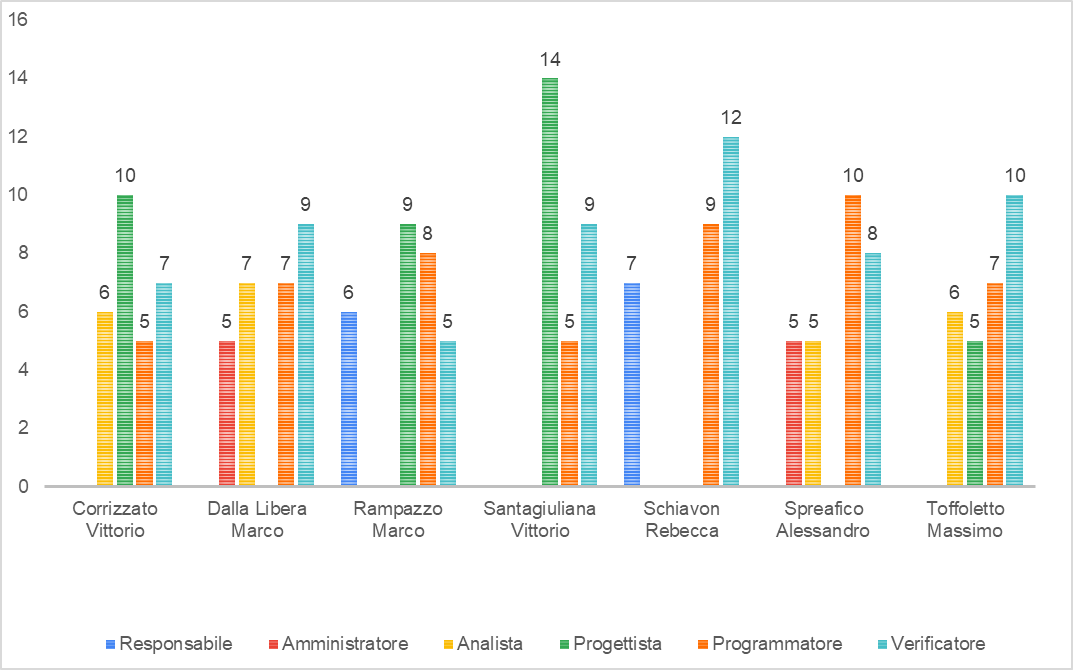
\includegraphics[width=\linewidth]{./img/Grafici/3.png}
		\caption{Grafico del prospetto orario del periodo di progettazione\glosp architetturale}
	\end{figure}

\subsubsection{Prospetto economico}
Nel periodo di progettazione\glosp architetturale sono previsti i seguenti costi:
\begin{longtable} {
		>{}p{32mm}
		>{}p{20mm}
		>{}p{20mm}
	}
	\rowcolor{gray!50}
	
	\textbf{Ruolo} & \textbf{Ore} & \textbf{Costo} \TBstrut \\
	Responsabile & 13 & 390,00\euro{} \TBstrut \\
	Amministratore & 10 & 200,00\euro{} \TBstrut \\
	Analista & 24 & 600,00\euro{} \TBstrut \\
	Progettista & 38 & 836,00\euro{} \TBstrut \\
	Programmatore & 51 & 765,00\euro{} \TBstrut \\
	Verificatore & 60 & 900,00\euro{} \TBstrut \\
	\textbf{Totale} & \textbf{196}& \textbf{3691,00\euro{}} \TBstrut \\	
	\rowcolor{white}
	\caption{Prospetto economico del periodo di progettazione architetturale}
\end{longtable}
\pagebreak
Rappresentati nel seguente grafico:
\begin{figure}[H] 
	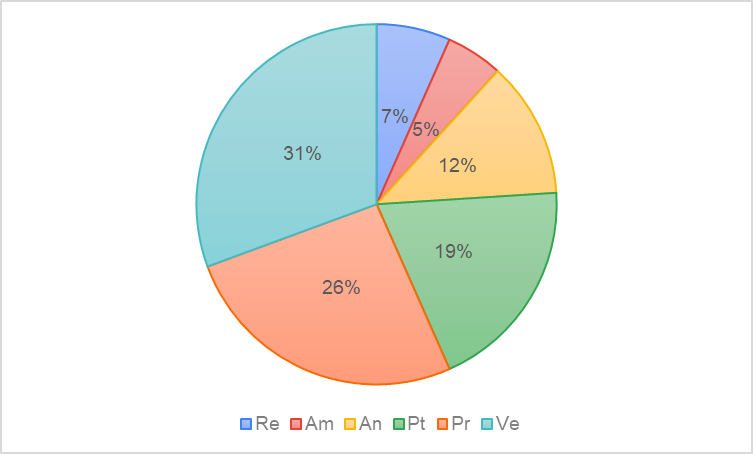
\includegraphics[width=\linewidth]{./img/Grafici/4.png}
	\caption{Grafico del prospetto economico del periodo di progettazione\glosp architetturale}
\end{figure}
\pagebreak
\subsection{Periodo di progettazione dettaglio e codifica}
\subsubsection{Prospetto orario}
Nel periodo di progettazione\glosp dettaglio e codifica è prevista la seguente divisione oraria:
\begin{longtable} {				
		>{}p{40mm}  
		>{}p{8mm}
		>{}p{8mm}
		>{}p{8mm}
		>{}p{8mm}
		>{}p{8mm}
		>{}p{8mm}
		>{}p{12mm}				
	}			
	\rowcolor{gray!50}
	\textbf{Nominativo} & \textbf{Re} & \textbf{Am} & \textbf{An} & \textbf{Pt} & \textbf{Pr} & \textbf{Ve} & \textbf{Totale}	\TBstrut \\ [2mm]
	Corrizzato Vittorio & - & - & 9 & 23 & 22 & - & 54 \TBstrut \\ [2mm]
	Dalla Libera Marco & 9 & - & 6 & 15 & 15 & 9 & 54 \TBstrut \\ [2mm]
	Rampazzo Marco & - & 5 & - & 23 & 18 & 8 & 54 \TBstrut \\ [2mm]
	Santagiuliana Vittorio & 8 & - & - & 20 & 15 & 11 & 54 \TBstrut \\ [2mm]
	Schiavon Rebecca & - & - & 8 & 20 & 18 & 8 & 54 \TBstrut \\ [2mm]
	Spreafico Alessandro & 8 & - & 0 & 16 & 18 & 12 & 54 \TBstrut \\ [2mm]
	Toffoletto Massimo & - & 5 & - & 23 & 15 & 11 & 54 \TBstrut \\ [2mm]
	\rowcolor{white}
	\caption{Prospetto orario del periodo di progettazione\glosp dettaglio e codifica}
\end{longtable}
\pagebreak
Rappresentata nel seguente grafico:
\begin{figure} [H]
	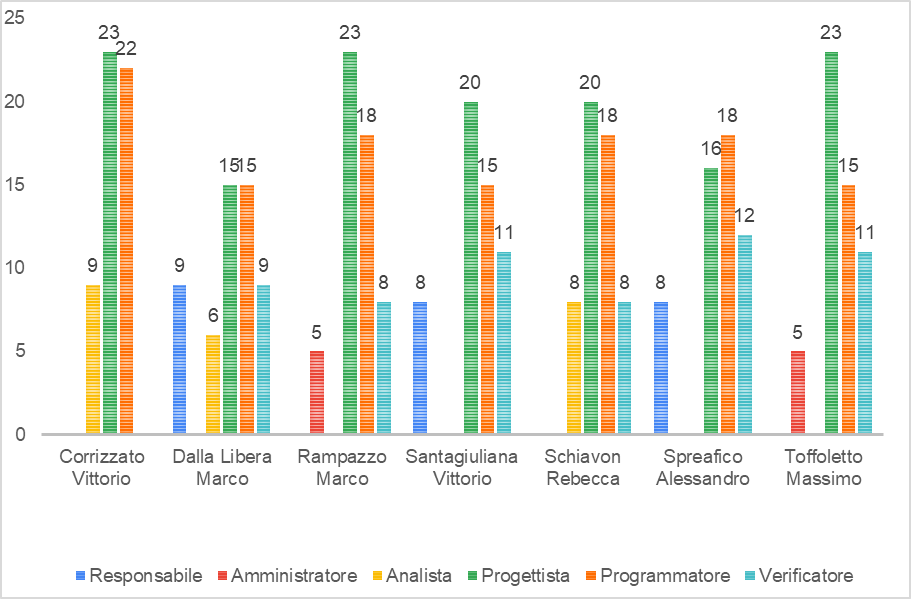
\includegraphics[width=\linewidth]{./img/Grafici/5.png}
	\caption{Grafico del prospetto orario del periodo di progettazione\glosp dettaglio e codifica}
\end{figure}
\subsubsection{Prospetto economico}
Nel periodo di progettazione\glosp dettaglio e codifica sono previsti i seguenti costi:
\begin{longtable} {
		>{}p{32mm}
		>{}p{20mm}
		>{}p{20mm}
	}
	\rowcolor{gray!50}
	
	\textbf{Ruolo} & \textbf{Ore} & \textbf{Costo} \TBstrut \\
	Responsabile & 25 & 750,00\euro{} \TBstrut \\
	Amministratore & 10 & 200,00\euro{} \TBstrut \\
	Analista & 23 & 575,00\euro{} \TBstrut \\
	Progettista & 140 & 3080,00\euro{}\TBstrut \\
	Programmatore & 121 & 1815,00\euro{} \TBstrut \\
	Verificatore & 59 & 885,00\euro{} \TBstrut \\
	\textbf{Totale} & \textbf{378}& \textbf{7305,00\euro{}} \TBstrut \\	
	\rowcolor{white}
	\caption{Prospetto economico del periodo di progettazione\glosp dettaglio e codifica}
\end{longtable} \mbox{} \\
Rappresentati nel seguente grafico: 
\begin{figure} [h!]
	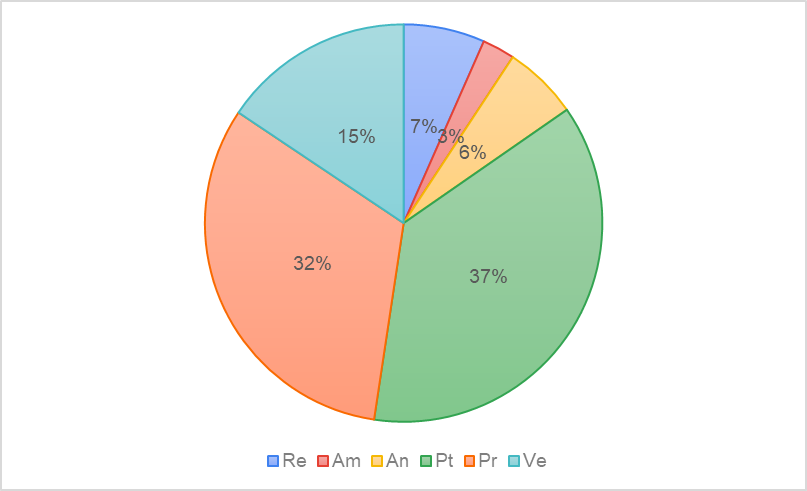
\includegraphics[width=\linewidth]{./img/Grafici/6.png}
	\caption{Grafico del prospetto economico del periodo di progettazione\glosp dettaglio e codifica}
\end{figure}

\subsection{Periodo di validazione e collaudo}
\subsubsection{Prospetto orario}
Nel periodo di validazione\glosp e collaudo è prevista la seguente divisione oraria:
\begin{longtable} {				
		>{}p{40mm}  
		>{}p{8mm}
		>{}p{8mm}
		>{}p{8mm}
		>{}p{8mm}
		>{}p{8mm}
		>{}p{8mm}
		>{}p{12mm}			
	}			
	\rowcolor{gray!50}
	\textbf{Nominativo} & \textbf{Re} & \textbf{Am} & \textbf{An} & \textbf{Pt} & \textbf{Pr} & \textbf{Ve} & \textbf{Totale}	\TBstrut \\ [2mm]
	Corrizzato Vittorio & - & - & - & - & 10 & 10 & 20 \TBstrut \\ [2mm]
	Dalla Libera Marco & 8 & 5 & - & - & 7 & - & 20 \TBstrut \\ [2mm]
	Rampazzo Marco & - & - & - & 5 & 8 & 7 & 20 \TBstrut \\ [2mm]
	Santagiuliana Vittorio & - & 5 & - & - & 6 & 9 & 20 \TBstrut \\ [2mm]
	Schiavon Rebecca & - & 8 & - & - & 7 & 5 & 20 \TBstrut \\ [2mm]
	Spreafico Alessandro & - & - & - & - & 8 & 12 & 20 \TBstrut \\ [2mm]
	Toffoletto Massimo & - & - & - & - & 9 & 11 & 20 \TBstrut \\ [2mm]
	\rowcolor{white}
	\caption{Prospetto orario del periodo di validazione\glosp e collaudo}
\end{longtable}
Rappresentata nel seguente grafico:
\begin{figure} [H]
	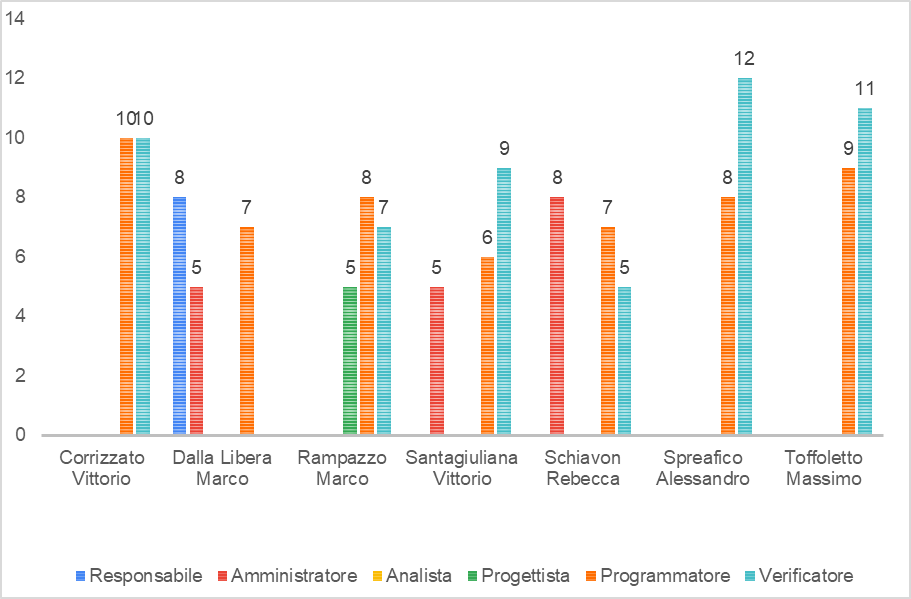
\includegraphics[width=\linewidth]{./img/Grafici/7.png}
	\caption{Grafico del prospetto orario del periodo di validazione\glosp e collaudo}
\end{figure}
\pagebreak
\subsubsection{Prospetto economico}
Nel periodo di validazione\glosp e collaudo sono previsti i seguenti costi:
\begin{longtable} {
		>{}p{32mm}
		>{}p{20mm}
		>{}p{20mm}
	}
	\rowcolor{gray!50}
	
	\textbf{Ruolo} & \textbf{Ore} & \textbf{Costo} \TBstrut \\
	Responsabile & 8 & 240,00\euro{} \TBstrut \\
	Amministratore & 18 & 360,00\euro{} \TBstrut \\
	Analista & 0 & 0,00\euro{} \TBstrut \\
	Progettista & 5 & 110,00\euro{} \TBstrut \\
	Programmatore & 55 & 825,00\euro{} \TBstrut \\
	Verificatore & 54 & 810,00\euro{} \TBstrut \\
	\textbf{Totale} & \textbf{140}& \textbf{2345,00\euro{}} \TBstrut \\	
	\rowcolor{white}
	\caption{Prospetto economico del periodo di validazione\glosp e collaudo}
\end{longtable}
Rappresentati nel seguente grafico:
\begin{figure} [H]
	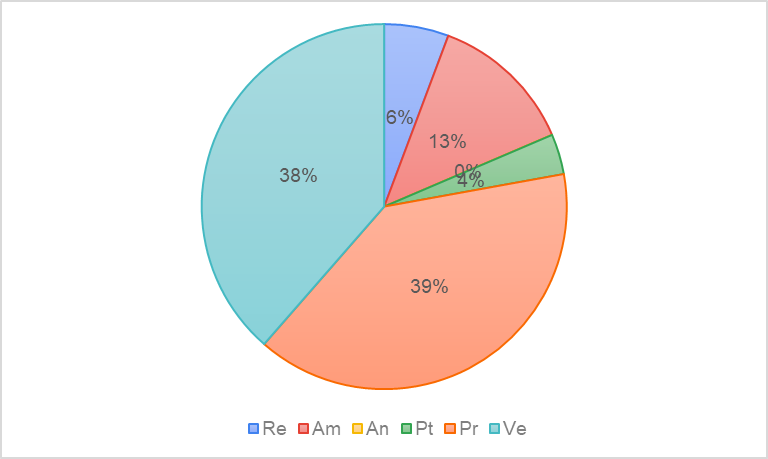
\includegraphics[width=\linewidth]{./img/Grafici/8.png}
	\caption{Grafico del prospetto economico del periodo di validazione \glosp e collaudo}
\end{figure}

\subsection{Totale ore investite}
\subsubsection{Prospetto orario}
La seguente tabella presenta la suddivisione delle ore investite per l'intero progetto\glo:
\begin{longtable} {				
		>{}p{40mm}  
		>{}p{8mm}
		>{}p{8mm}
		>{}p{8mm}
		>{}p{8mm}
		>{}p{8mm}
		>{}p{8mm}
		>{}p{12mm}			
	}			
	\rowcolor{gray!50}
	\textbf{Nominativo} & \textbf{Re} & \textbf{Am} & \textbf{An} & \textbf{Pt} & \textbf{Pr} & \textbf{Ve} & \textbf{Totale}	\TBstrut \\ [2mm]
	Corrizzato Vittorio & 6 & 6 & 23 & 33 & 37 & 22 & 127 \TBstrut \\ [2mm]
	Dalla Libera Marco & 24 & 10 & 26 & 15 & 29 & 23 & 127 \TBstrut \\ [2mm]
	Rampazzo Marco & 6 & 13 & 12 & 37 & 34 & 25 & 127 \TBstrut \\ [2mm]
	Santagiuliana Vittorio & 8 & 10 & 12 & 34 & 26 & 37 & 127 \TBstrut \\ [2mm]
	Schiavon Rebecca & 7 & 8 & 23 & 20 & 34 & 35 & 127 \TBstrut \\ [2mm]
	Spreafico Alessandro & 8 & 5 & 17 & 21 & 36 & 40 & 127 \TBstrut \\ [2mm]
	Toffoletto Massimo & 8 & 12 & 11 & 28 & 31 & 37 & 127 \TBstrut \\ [2mm]
	\rowcolor{white}
	\caption{Prospetto orario del totale di ore investite}
\end{longtable}
\pagebreak
Rappresentata anche nel seguente grafico:
\begin{figure} [H]
	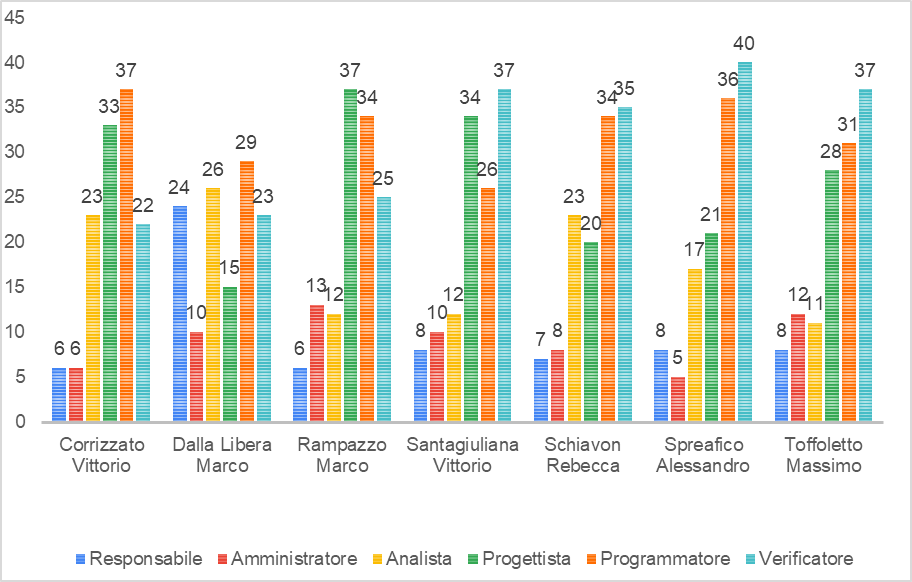
\includegraphics[width=\linewidth]{./img/Grafici/9.png}
	\caption{Grafico del prospetto orario delle ore investite per l'intero progetto\glo}
\end{figure}

\subsubsection{Prospetto economico}
La seguente tabella presenta i costi delle ore investite per l'intero progetto\glo:
\begin{longtable} {
		>{}p{32mm}
		>{}p{20mm}
		>{}p{20mm}
	}
	\rowcolor{gray!50}
	
	\textbf{Ruolo} & \textbf{Ore} & \textbf{Costo} \TBstrut \\
	Responsabile & 67 & 2010,00\euro{} \TBstrut \\
	Amministratore & 64 & 1280,00\euro{} \TBstrut \\
	Analista & 124 & 3100,00\euro{} \TBstrut \\
	Progettista & 188 & 4136,00\euro{} \TBstrut \\
	Programmatore & 227 & 3405,00\euro{} \TBstrut \\
	Verificatore & 219 & 3285,00\euro{} \TBstrut \\
	\textbf{Totale} & \textbf{749}& \textbf{17216,00\euro{}} \TBstrut \\		
	\rowcolor{white}
	\caption{Prospetto economico del totale di ore investite}
\end{longtable} \mbox{} \\ \\ \\
Rappresentati anche nel seguente grafico:
\begin{figure} [H]
	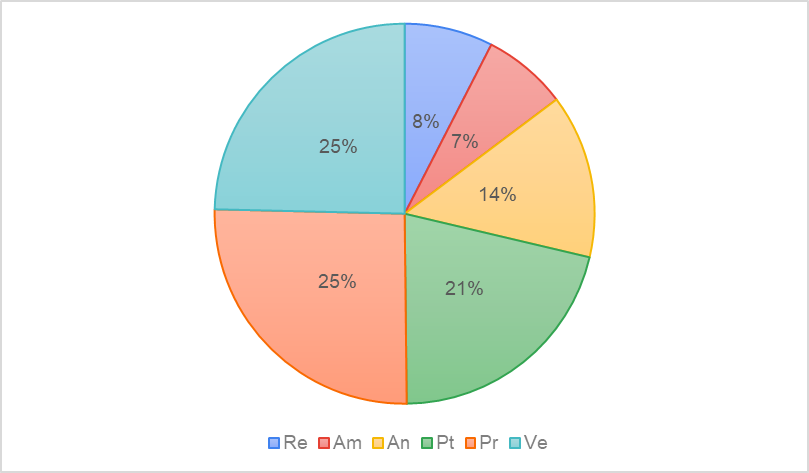
\includegraphics[width=\linewidth]{./img/Grafici/10.png}
	\caption{Grafico del prospetto economico delle ore investite per l'intero progetto\glo}
\end{figure}

\subsection{Totale ore rendicontate}
\subsubsection{Prospetto orario}
La seguente tabella presenta la suddivisione delle ore rendicontate per l'intero progetto\glo:
\begin{longtable} {				
		>{}p{40mm}  
		>{}p{8mm}
		>{}p{8mm}
		>{}p{8mm}
		>{}p{8mm}
		>{}p{8mm}
		>{}p{8mm}
		>{}p{12mm}			
	}			
	\rowcolor{gray!50}
	\textbf{Nominativo} & \textbf{Re} & \textbf{Am} & \textbf{An} & \textbf{Pt} & \textbf{Pr} & \textbf{Ve} & \textbf{Totale}	\TBstrut \\ [2mm]
	Corrizzato Vittorio & - & - & 15 & 33 & 37 & 17 & 102 \TBstrut \\ [2mm]
	Dalla Libera Marco & 17 & 10 & 13 & 15 & 29 & 18 & 102 \TBstrut \\ [2mm]
	Rampazzo Marco & 6 & 5 & - & 37 & 34 & 20 & 102 \TBstrut \\ [2mm]
	Santagiuliana Vittorio & 8 & 5 & - & 34 & 26 & 29 & 102 \TBstrut \\ [2mm]
	Schiavon Rebecca & 7 & 8 & 8 & 20 & 34 & 25 & 102 \TBstrut \\ [2mm]
	Spreafico Alessandro & 8 & 5 & 5 & 16 & 36 & 32 & 102 \TBstrut \\ [2mm]
	Toffoletto Massimo & - & 5 & 6 & 28 & 31 & 32 & 102 \TBstrut \\ [2mm]
	\rowcolor{white}
	\caption{Prospetto orario del totale di ore rendicontate}
\end{longtable}
Rappresentata anche nel seguente grafico:
\begin{figure} [H]
	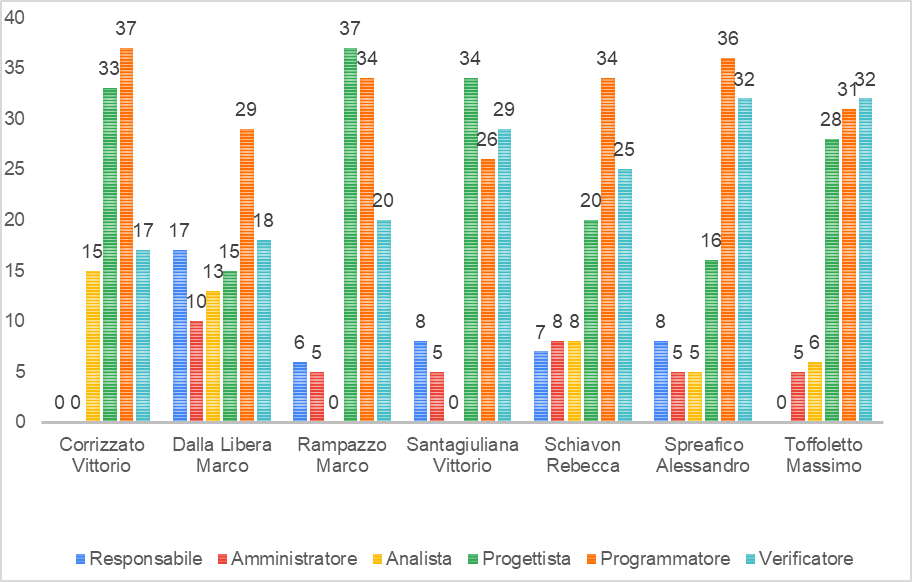
\includegraphics[width=\linewidth]{./img/Grafici/11.png}
	\caption{Grafico del prospetto orario delle ore rendicontate per l'intero progetto\glo}
\end{figure}
\pagebreak
\subsubsection{Prospetto economico}
La seguente tabella presenta i costi delle ore rendicontate per l'intero progetto\glo
\begin{longtable} {
		>{}p{32mm}
		>{}p{20mm}
		>{}p{20mm}
	}
	\rowcolor{gray!50}
	
	\textbf{Ruolo} & \textbf{Ore} & \textbf{Costo} \TBstrut \\
	Responsabile & 46 & 1380,00\euro{} \TBstrut \\
	Amministratore & 38 & 760,00\euro{} \TBstrut \\
	Analista & 47 & 1175,00\euro{} \TBstrut \\
	Progettista & 183 & 4026,00\euro{} \TBstrut \\
	Programmatore & 227 & 3405,00\euro{} \TBstrut \\
	Verificatore & 173 & 2595,00\euro{} \TBstrut \\
	\textbf{Totale} & \textbf{714}& \textbf{13341,00\euro{}} \TBstrut \\		
	\rowcolor{white}
	\caption{Prospetto economico del totale di ore rendicontate}
\end{longtable} \mbox{} \\ \\
Rappresentati anche nel seguente grafico:
\begin{figure} [H]
	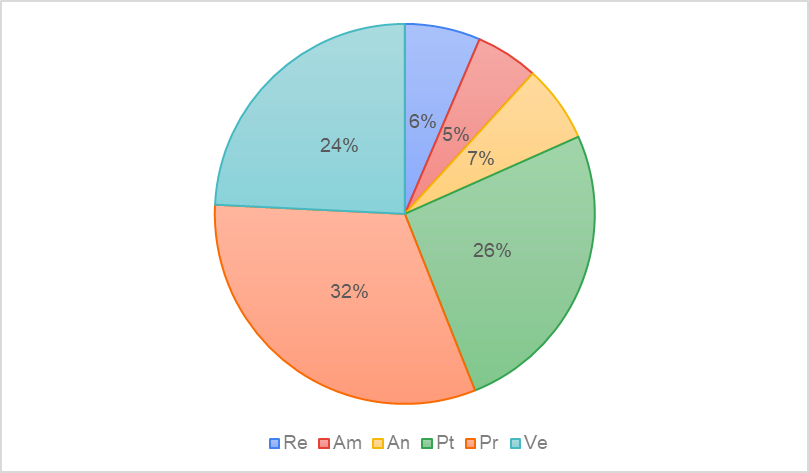
\includegraphics[width=\linewidth]{./img/Grafici/12.png}
	\caption{Grafico del prospetto economico delle ore rendicontate per l'intero progetto\glo}
\end{figure}
	
\section{Consuntivi di periodo}
Vengono riportati gli effettivi costi sostenuti per ogni periodo con le eventuali differenze rispetto a quanto preventivato. Il bilancio risulterà quindi:
\begin{itemize}
	\item \textbf{Positivo}: se i costi del consuntivo risultano minori di quelli del preventivo;
	\item \textbf{Pari}: se i costi del consuntivo risultano uguali a quelli del preventivo;
	\item \textbf{Negativo}: se i costi del consuntivo risultano superiori a quelli del preventivo.
\end{itemize}
Seguiranno quindi le conclusioni con le motivazioni delle eventuali differenze e le contromisure che il gruppo ha deciso di attuare per evitare ulteriori discrepanze con quanto dichiarato nel preventivo.
	\subsection{Periodo di Analisi}
	La tabella riporta il numero di ore effettivamente svolte dal gruppo e il rispettivo costo con le eventuali differenze rilevate rispetto al preventivo
	\begin{longtable} {							
			>{}p{40mm}  
			>{}p{20mm}	
			>{}p{28mm}			
		}			
		\rowcolor{gray!50}
		
		\textbf{Ruolo} & \textbf{Ore} & \textbf{Costo} \TBstrut \\
		Responsabile & 20(-1) & 600\euro{}(-30\euro{}) \TBstrut \\
		Amministratore & 26 & 520\euro{} \TBstrut \\
		Analista & 86(+9)& 2150\euro{}(+225\euro{}) \TBstrut \\
		Progettista & 10(+5) & 220\euro{}(+110\euro{}) \TBstrut \\
		Programmatore & 0 & 0\euro{} \TBstrut \\
		Verificatore & 46 & 690\euro{} \TBstrut \\
		\textbf{Totale Preventivo} & 175 & 3875\euro{}	\TBstrut \\	
		\textbf{Totale Consuntivo} & 188 & 4180\euro{}	\TBstrut \\	
		\textbf{Differenza Totale} & +13 & +305\euro{} \TBstrut \\
		\rowcolor{white}
		\caption{Numero di ore effettivamente svolte con rispettivo costo e differenze rispetto al preventivo}	
	\end{longtable}
	\pagebreak
	Rappresentate anche dai grafici:
	\begin{figure} [H]
		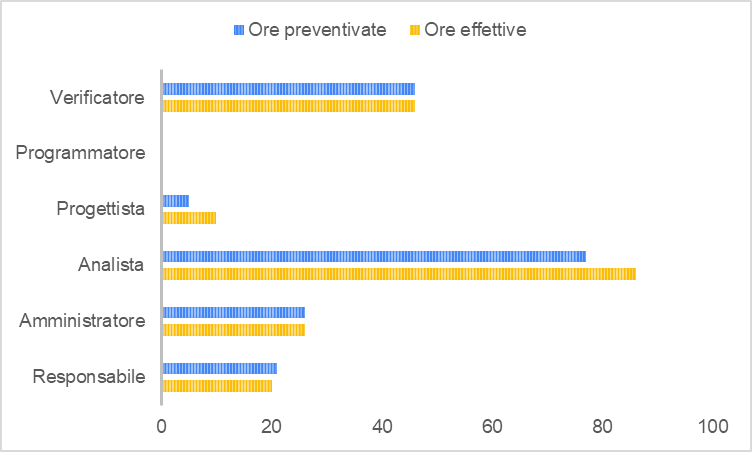
\includegraphics[width=\linewidth]{./img/Grafici/13.png}
		\caption{Grafico delle ore preventivate rispetto alle ore effettive}
	\end{figure}

	\begin{figure} [H]
		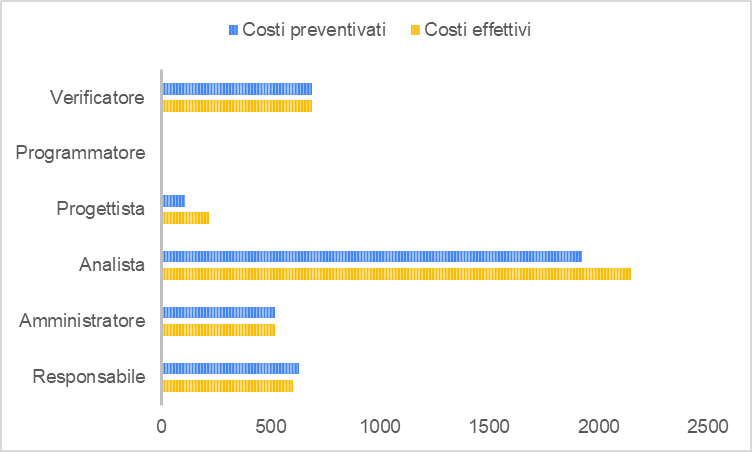
\includegraphics[width=\linewidth]{./img/Grafici/14.png}
		\caption{Grafico dei costi preventivati rispetto ai costi effettivi}
	\end{figure}

		\subsubsection{Conclusioni}
		Il bilancio risulta negativo perché le ore effettivamente svolte nei ruoli di analista, progettista e verificatore hanno superato le ore previste dal preventivo.
		Le motivazioni che hanno portato alla necessità di lavorare più del previsto sono le seguenti:
		\begin{itemize}
			\item \textbf{Analisiti}: la stesura dell'\textit{Analisi dei Requisiti} è risultata più complessa del previsto in particolare nell'individuazione dei casi d'uso\glosp e dei requisiti;
			\item \textbf{Progettisti}: sono sorte complicazioni non preventivate nella stesura del \textit{Piano di Qualifica} che hanno portato alla necessità di svolgere maggiore attività di autoapprendimento e ad un conseguente rallentamento del lavoro.
		\end{itemize}
		\subsubsection{Preventivo a finire}
		Il periodo di analisi è da intendersi come periodo di investimento per il gruppo e non viene quindi rendicontato, nel budget finale la variazione tra le ore previste e le ore effettive non provocherà alcun cambiamento. 
		È stato inoltre deciso di non modificare i successivi prospetti orari in quanto le condizioni che hanno portato alla necessità di lavorare più di quanto preventivato non dovrebbero presentarsi nuovamente. Il gruppo si ritiene ora più consapevole e meglio preparato, grazie anche alle ore di autoapprendimento già effettuate, e continua a considerare ragionevoli i prospetti orari dei prossimi periodi.
		
		\pagebreak
		\subsection{Periodo di progettazione architetturale}
		La tabella riporta il numero di ore effettivamente svolte dal gruppo e il rispettivo costo con le eventuali differenze rilevate rispetto al preventivo
		\begin{longtable} {							
				>{}p{40mm}  
				>{}p{20mm}	
				>{}p{28mm}			
			}			
			\rowcolor{gray!50}
			
			\textbf{Ruolo} & \textbf{Ore} & \textbf{Costo} \TBstrut \\
			Responsabile & 14(+1) & 420\euro (+30\euro) \TBstrut \\
			Amministratore & 13(+3) & 260\euro (+60\euro)\TBstrut \\
			Analista & 22(-2) & 550\euro (-50\euro) \TBstrut \\
			Progettista & 38 & 836\euro \TBstrut \\
			Programmatore & 58(+7) & 870\euro (+105\euro) \TBstrut \\
			Verificatore & 60 & 900\euro \TBstrut \\
			\textbf{Totale Preventivo} & 196 & 3691\euro	\TBstrut \\	
			\textbf{Totale Consuntivo} & 205 & 3836\euro	\TBstrut \\	
			\textbf{Differenza Totale} & +9 & +145\euro \TBstrut \\
			\rowcolor{white}
			\caption{Numero di ore effettivamente svolte con rispettivo costo e differenze rispetto al preventivo}	
		\end{longtable}
		Rappresentate anche dai grafici:
		\begin{figure} [H]
			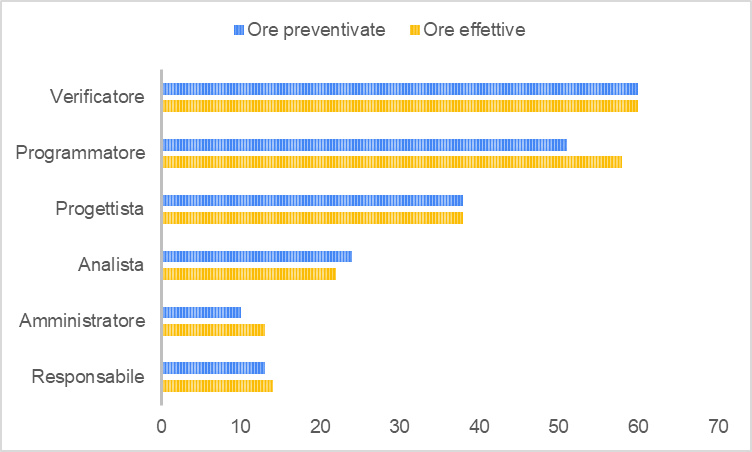
\includegraphics[width=\linewidth]{./img/Grafici/15.png}
			\caption{Grafico delle ore preventivate rispetto alle ore effettive}
		\end{figure}
		
		\begin{figure} [H]
			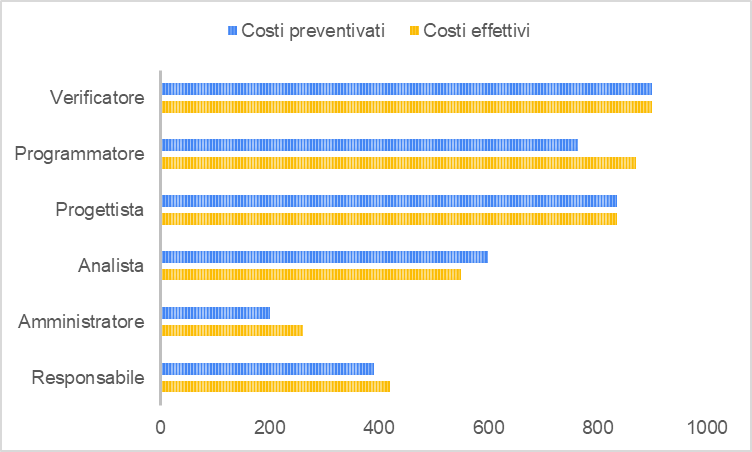
\includegraphics[width=\linewidth]{./img/Grafici/16.png}
			\caption{Grafico dei costi preventivati rispetto ai costi effettivi}
		\end{figure}
		\subsubsection{Analisi degli scostamenti}
		Al fine di garantire uno sviluppo del progetto\glosp congruo con quanto preventivato nei tempi e nei costi, al termine di ogni periodo individuato nella pianificazione si rilevano eventuali problemi riscontrati ed eventualmente si modifica e si dettaglia ulteriormente la pianificazione futura in modo da mitigare gli effetti di questi imprevisti.
		\paragraph*{I periodo} \mbox{} \\
		Il tempo dedicato alla revisione e all'aggiornamento delle \textit{Norme di Progetto} è risultato insufficiente, è stato quindi necessario prolungare quest'attività anche per il secondo periodo.
		Ciò ha causato un aumento delle ore del ruolo dell'amministratore.
		\paragraph*{II periodo} \mbox{} \\
		Al termine del secondo periodo non è stata individuata nessuna complicazione. Nonostante si sia dovuta rivedere la pianificazione vista la necessità di inserire anche in questo periodo l'attività di revisione e aggiornamento delle \textit{Norme di Progetto}, non sono stati rilevati ritardi o imprevisti oltre all'aumento delle ore per il ruolo dell'amministratore come già indicato. È stata quindi mantenuta la pianificazione prevista per il III periodo.
		\paragraph*{III periodo} \mbox{} \\
		È stato rilevato che l'attività di ricerca di strumenti e tecnologie svolta nel I periodo non è stata affiancata da un sufficiente studio degli strumenti e delle tecnologie individuate. Questo ha portato alla necessità di svolgere dell'autoapprendimento da parte di due componenti del gruppo che hanno poi illustrato quanto appreso agli altri membri. Di conseguenza si è verificato un ritardo nel ruolo dei programmatori. Questo ritardo, tuttavia, non è stato così rilevante da non permettere la codifica del proof of concept\glosp come da pianificazione, non è stato quindi necessario nessun cambiamento sulla pianificazione futura. 
		\paragraph*{IV periodo} \mbox{} \\
		Grazie all'attività di autoapprendimento svolta nel III periodo non ci sono stati problemi o ritardi nel IV periodo.
		\paragraph*{V periodo} \mbox{} \\
		Non sono stati rilevati scostamenti dalla pianificazione del V periodo.
		\subsubsection{Conclusioni}
		Il bilancio risulta negativo perché le ore effettivamente svolte nei ruoli di responsabile, amministratore e programmatore hanno superato le ore previste dal preventivo.
		Le motivazioni che hanno portato alla necessità di lavorare più del previsto sono le seguenti:
		\begin{itemize}
			\item \textbf{Responsabile}: per cause di forza maggiore, esterne all'ambito universitario, è stato impossibile svolgere alcuni incontri previsti ed è stata necessaria una conseguente riorganizzazione delle modalità di incontro, ciò ha portato ad un inatteso aumento del lavoro per il responsabile;
			\item \textbf{Amministratore}: è sorta la necessità di utilizzare strumenti e tecnologie inizialmente non previsti, la necessità di normare l'utilizzo di quest'ultimi ha rallentato la revisione e l'aggiornamento delle \textit{Norme di Progetto} richiedendo un aumento delle ore lavorative per l'amministratore;
			\item \textbf{Programmatore}: è stato necessario uno studio più approfondito delle tecnologie rispetto a quanto non era già stato preventivato, ciò ha causato la necessità di un numero maggiore di ore anche per i programmatori.
		\end{itemize}
		Le contromisure attuate per mitigare i problemi riscontrati sono indicate nell'analisi degli scostamenti e nelle tabelle di attuazione dei rischi.
		\subsubsection{Preventivo a finire}
		Il bilancio risulta negativo in quanto i costi effettivi superano quelli preventivati. Per fronteggiare questo problema verrà modificata la pianificazione futura in modo da presentarci ai proponenti con un preventivo finale il più aderente possibile a quello iniziale. 

	\pagebreak
	\renewcommand{\thesection}{\alph{section}}
\section{Riscontro dei rischi}
    \subsection{Attualizzazione dei rischi 2020-01-14}
        \rowcolors{2}{gray!25}{gray!15}
	    \begin{longtable} {
		    >{}p{24mm} 
		    >{}p{32mm}
		    >{}p{40mm} 
            >{}p{40mm}
		    }
	    \rowcolor{gray!50}
        \textbf{ID} & \textbf{Tempistiche} & \textbf{Descrizione} & \textbf{Manutenzione migliorativa}	\TBstrut \\
        RT1 & Creazione del template \LaTeX e della repository\glo & Nella prima fase del progetto\glosp ci sono state difficoltà dovute all'apprendimento di \LaTeX, il cui funzionamento era sconosciuto a tutti i membri del gruppo, e alla gestione di GitHub, noto a tutti i componenti, ma mai utilizzato al pieno delle sue possibilità & Per quanto riguarda \LaTeX è stato necessario un breve periodo di autoapprendimento da parte di alcuni componenti del gruppo, mentre per GitHub i membri del gruppo che hanno partecipato al corso di Tecnologie Open Source hanno contribuito a proporre delle soluzioni studiate a lezione  \TBstrut \\ [2mm]
        RG1 & \textit{Glossario} & È stato oggetto di una lunga discussione il metodo di stesura del \textit{Glossario}, soprattutto la scelta dei termini da inserire in esso & Alla fine di una condivisione di opinioni il responsabile ha delineato delle linee guida per la scelta dei lemmi da inserire nel \textit{Glossario} che hanno messo d'accordo i componenti del gruppo \TBstrut \\ [2mm]
        RG2 & Rischio permanente & I membri del gruppo sono dovuti andare incontro ad inevitabili sovrapposizioni di impegni durante la stesura dei documenti, tale rischio ha influenzato l'incidenza di RS1 & Ogni componente, per quanto possibile, ha cercato di ritagliarsi del tempo per rispettare le milestone e, eventualmente, ha chiesto assistenza ad altri componenti più disponibili \TBstrut \\ [2mm]
        RO2 & Gestione della repository\glo & Collegandosi a RT1 la scarsa esperienza nell'utilizzo di GitHub ha generato lacune nella corretta gestione dell'issue tracking system integrato nella piattaforma & I membri del gruppo che hanno seguito il corso di Tecnologie Open Source, e quindi più pratici nei sistemi di versionamento\glo, hanno risolto le inconsistenze individuate in GitHub \TBstrut \\ [2mm]
        RO3 & Stesura primi documenti & Con la stesura dei primi documenti alcuni componenti hanno trovato difficoltà ad adattarsi ai vari ruoli assegnati & I membri del gruppo si sono assistiti a vicenda cercando di colmare le debolezze evidenziate sotto certi aspetti dando delle linee guida sui processi\glosp di analisi e di verifica dei documenti \TBstrut \\ [2mm]
        RR1 & \textit{Studio di Fattibilità} e \textit{Analisi dei Requisiti} & Non avendo esperienza sugli strumenti da utilizzare certe specifiche richieste non sono state chiare o sono state mal interpretate & Per ovviare a questo problema sono stati indetti due incontri con il proponente che hanno contribuito a risolvere i dubbi sorti durante l'analisi dei documenti \TBstrut \\ [2mm]
        RS1 & Rischio permanente & Data la scarsa esperienza nella gestione di una tale mole di lavoro e gli impegni personali dei componenti certe milestone sono risultate imprecise e difficilmente rispettabili & Pur essendo stato un problema persistente man mano si è diminuita l'imprecisione delle scadenze inoltre, il proseguimento del lavoro in gruppo dovrebbe portare ad avere maggiore consapevolezza dei tempi e quindi il calo di incidenza del rischio \TBstrut \\ [2mm]
        \rowcolor{white}
        \caption{Attualizzazione dei rischi 2020-01-14}
        \end{longtable}
	\pagebreak
	\section{Organigramma}
	\subsection{Redazione}
	
	\rowcolors{2}{gray!25}{gray!15}
	\begin{longtable} {
			>{\centering}m{40mm} %m al posto di p sembra centrare verticalmente il testo
			>{\centering}m{19.5mm}
			>{}m{70mm}}
		
		\rowcolor{gray!50}
		\textbf{Nome} & \textbf{Data} & \textbf{Firma}   \TBstrut \\
		Vittorio Corrizzato  & 08/01/2020 & 
\includegraphics[scale=0.3]{../../../images/firme/sfondo_trasparente/firma-trasparente-VittorioC.png}   \TBstrut  \\ %qui ho aggiunto un'immagine tanto per vedere se funzionava
		\rowcolor{white}
		\caption{Redazione}
	\end{longtable}
	
	\subsection{Approvazione}
	
	\rowcolors{2}{gray!25}{gray!15}
	\begin{longtable} {
			>{\centering}m{40mm} 
			>{\centering}m{19.5mm}
			>{}m{70mm}}
		
		\rowcolor{gray!50}
		\textbf{Nome} & \textbf{Data} & \textbf{Firma}      \TBstrut \\
		Rebecca Schiavon       & 08/01/2020 & 
\includegraphics[scale=0.3]{../../../images/firme/sfondo_trasparente/firma-trasparente-RebeccaS.png}    \TBstrut  \\  
		Prof Riccardo Cardin   & 		    &   				\TBstrut  \\ [0.82cm]
		Prof Tullio Vardanega  & 	        & 				\TBstrut  \\  [0.82cm]
		\rowcolor{white}
		\caption{Approvazione}
	\end{longtable}
	
	\subsection{Accettazione dei componenti}
	
	\rowcolors{2}{gray!25}{gray!15}
	\begin{longtable} {
			>{\centering}m{40mm} 
			>{\centering}m{19.5mm}
			>{}m{70mm}}
		
		\rowcolor{gray!50}
		\textbf{Nome} & \textbf{Data} & \textbf{Firma}   \TBstrut \\
		Vittorio Corrizzato    & 08/01/2020 & 
\includegraphics[scale=0.3]{../../../images/firme/sfondo_trasparente/firma-trasparente-VittorioC.png}  \TBstrut  \\
		Marco Dalla Libera     & 08/01/2020 & 
\includegraphics[scale=0.3]{../../../images/firme/sfondo_trasparente/firma-trasparente-MarcoD.png}  \TBstrut  \\
		Marco Rampazzo         & 08/01/2020 & 
\includegraphics[scale=0.3]{../../../images/firme/sfondo_trasparente/firma-trasparente-MarcoR.png}   \TBstrut  \\
		Vittorio Santagiuliana & 08/01/2020 & 
\includegraphics[scale=0.3]{../../../images/firme/sfondo_trasparente/firma-trasparente-VittorioS.png}   \TBstrut  \\
		Rebecca Schiavon       & 08/01/2020 & 
\includegraphics[scale=0.3]{../../../images/firme/sfondo_trasparente/firma-trasparente-RebeccaS.png}  \TBstrut  \\
		Alessandro Spreafico   & 08/01/2020 & 
\includegraphics[scale=0.3]{../../../images/firme/sfondo_trasparente/firma-trasparente-AlessandroS.png}   \TBstrut  \\ 
		Massimo Toffoletto     & 08/01/2020 & 
\includegraphics[scale=0.3]{../../../images/firme/sfondo_trasparente/firma-trasparente-MassimoT.png}   \TBstrut  \\
		\rowcolor{white}
		\caption{Accettazione dei componenti}
	\end{longtable}
	
	\subsection{Componenti}
	
		\rowcolors{2}{gray!25}{gray!15}
	\begin{longtable} {
			>{\centering}m{40mm} 
			>{\centering}m{18.5mm}
			>{}m{73mm}}
		
		\rowcolor{gray!50}
		\textbf{Nome} & \textbf{Matricola} & \textbf{Email}   \TBstrut \\
		Vittorio Corrizzato    & 1122288 & vittorio.corrizzato@studenti.unipd.it     \TBstrut  \\ [0.2cm]
		Marco Dalla Libera     & 1170634 & marco.dallalibera.2@studenti.unipd.it     \TBstrut  \\ [0.2cm]
		Marco Rampazzo         & 1170754 & marco.rampazzo.10@studenti.unipd.it       \TBstrut  \\ [0.2cm]
		Vittorio Santagiuliana & 1170542 & vittorio.santagiuliana@studenti.unipd.it  \TBstrut  \\ [0.2cm]
		Rebecca Schiavon       & 1163774 & rebecca.schiavon@studenti.unipd.it        \TBstrut  \\ [0.2cm]
		Alessandro Spreafico   & 1148755 & alessandro.spreafico@studenti.unipd.it    \TBstrut  \\ [0.2cm]
		Massimo Toffoletto     & 1161727 & massimo.toffoletto@studenti.unipd.it      \TBstrut  \\ [0.2cm]
		\rowcolor{white}
		\caption{Componenti}
	\end{longtable}
	
	%Input del file "decision_table" della cartella locale "res/"
	%% \textbf = grassetto; \Large = font più grande
% \rowcolors{quanti colori alternare}{colore numero riga pari}{colore numero riga dispari}: colori alternati per riga
% \rowcolor{color}: cambia colore di una riga
% p{larghezza colonna}: p è un tipo di colonna di testo verticalmente allineata sopra, ci sarebbe anche m che è centrata a metà ma non è precisa per questo utilizzo TBStrut; la sintassi >{\centering} indica che il contenuto della colonna dovrà essere centrato
% \TBstrut fa parte di alcuni comandi che ho inserito in config.tex che permetto di aggiungere un po' di padding al testo
% \\ [2mm] : questra scrittura indica che lo spazio dopo una break line deve essere di 2mm

%\setcounter{secnumdepth}{0}
%\hfill \break
%\textbf{\Large{Diario delle modifiche}} \\
\section{Riepilogo tracciamenti}
\rowcolors{2}{gray!25}{gray!15}
\begin{longtable} {
		>{\centering}p{17mm} 
		%>{\centering}p{19.5mm}
		%>{\centering}p{24mm} 
		%>{\centering}p{24mm} 
		>{}p{120mm}}
	\rowcolor{gray!50}
	\textbf{Codice} & \multicolumn{1}{c}{\textbf{Decisione}} \\%\textbf{Decisione} \\ %\TBstrut \\
	VI\_1.1 & Scelto \textit{VRAM Software} come nome del gruppo. \TBstrut \\ [2mm]
	VI\_1.1 & Scelto \textit{VRAM Software} come nome del gruppo. \TBstrut \\ [2mm]
	VI\_1.1 & Scelto \textit{VRAM Software} come nome del gruppo. \TBstrut \\ [2mm]
	
\end{longtable} %Tabella delle decisioni (solo per i verbali)
\end{document}